\begin{savequote}[8cm]
Energy can neither be created nor destroyed \\
Matter can neither be created nor destroyed \\
Every atom in my body goes back to the Big Bang \\
So rap is no big thang, I was created in the void
  \qauthor{---  Grip Grand, \textit{Conservation of Matter}}
\end{savequote}

\chapter{\label{ch:6-defects}H-centre defects}

\section{Introduction}

Until this point we have considered a lattice with perfect translational symmetry and no missing or extra atoms. However at finite temperature a crystalline material always contains point defects, as the cost in lattice energy is balanced by the increase in configurational entropy.
In this chapter we consider the iodine interstitial defect and predict that it will form a split-interstitial defect with self-trapped hole ($\mathrm{I}_\mathrm{i}^-+\mathrm{I}_\mathrm{i}^-+\mathrm{h}^+ \rightarrow \mathrm{I}_\mathrm{2}^-$). The vibrational properties of the defect are studied to i) confirm the validity of the 1D configurational coordinate approach and ii) predict the electron capture coefficient at this defect site.

As outlined briefly in Section \ref{recombination} we are often interested in semiconductor defects that form electronic states in the bandgap, as these can provide sites for non-radiative processes such as minority carrier trapping and electron-hole recombination, both of which limit the photovoltaic efficiency of solar cell absorber materials. Marshall Stoneham coined the term `killer centre' for defects with fast non-radiative transitions and lists the defect types that may act as performance killers. Two of four in the list relate to the vibrational properties of the defect lattice:

\begin{displayquote}
``2. Defects with favorable vibrational properties, that is, with large-amplitude modes promoting the transitions, and large-energy modes to take up the electronic energy.

3.  Defects with very strong coupling to lattice distortions such as certain dislocations and some vacancy centers.''
\end{displayquote}

However historically there has been increased research emphasis on the electronic properties of `killer centres', as the calculations required to predict the vibrational properties of imperfect crystals from first principles are computationally demanding.
With recent advances in first principles modelling \autocite{Alkauskas2014}%also sunghyun's paper an dalkauskas review 
and the growth in available computing power\autocite{}
it is now possible to calculate from first principles the coupling strength between the electronic states of the defect and bulk phonons to predict the rate of carrier capture and recombination for systems of interest. 
This methodology has been recently applied to \ce{CZTS} where it has been found that the sulfur vacancy provides a site for fast non-radiative recombination.

Hybrid halide perovskite materials are often classed in the literature as `defect tolerant' materials with low concentration of killer defects. This is for two reasons. 
Firstly, good device performance can be achieved using a low-temperature solution processing method which is expected to form a thin film with a high concentration of defects. 
%For example, the $V_\mathrm{oc}$ deficit for solution processed hybrid halide perovskite materials can be as low as \SI{0.5}{\volts}, compared to 
%http://www.nature.com/articles/srep06071
Secondly, theoretical calculations show that Schottky and Frenkel point defects form at high concentrations, but that they form electronic states either in the electronic bands or at shallow energies in the bandgap ($< \mathrm{kT}$ from the band edge) and so are unlikely to contribute to non-radiative recombination.
%Self-Regulation Mechanism for Charged Point Defects in Hybrid Halide Perovskites** Aron Walsh,* 
%  (http://pubs.acs.org/doi/ipdf/10.1021/jz500370k)
Amongst the native non-stochiometric defects in MAPI the iodine interstitial is predicted to be the only stable and active trap species.
%cite de angelis
% Several studies42,43 have taken advantage of absorption and emission reciprocity relationships in complete solar cells to show that the predominant contribution to the deficit in VOC from its ideal value under solar illumination is a low EQEEL value. This indicates that most carriers recombine non-radiatively. These relationships have been recently explored in mixed-cation, mixed-halide perovskites, concluding that the EQEEL is limited by SRH recombination in devices with state-of-the-art power conversion efficiency44. % https://www.nature.com/articles/nenergy2016149



The halide sub-lattice is also associated with ionic migration, with iodine ions being the dominant mobile species in MAPI. %The nature of ion conduction in methylammonium lead iodide: a multimethod approach
Experimental evidence points to a coupling between the electronic and ionic states, and various models exist which link trapping at the iodine ion with phase segregation and hysterisis in hybrid halide perovskites.
This has motivated the recent research interest in the point defect properties of halide perovskites, and in the properties of the iodine interstitial in particular.
% talk about photoinduced brightening as it will come in again later: https://www.nature.com/articles/ncomms11683
% Even though the shallow level point defects donot contribute to non-radiative recombination, their ionic natureenables them to migrate within an electric field.
% comment that this is not just for deep but for shallow also

Point defects in hybrid halide perovskites are a challenge to model from first principles. Due to the organic cation the structure is low symmetry and there are three inequivalent iodine sites. The atomic lattice is soft and distorts easily, often requiring hundreds of ionic steps to achieve force convergence. 
Previous calculations in the literature demonstrate that the defect formation energies are sensitive to the level of theory used; hybrid functionals with spin-orbit coupling predict electrically active charge states of the iodine interstitial that are not found at lower levels of theory.
%mao hua du
Furthermore, comparison with experiment remains a challenge. Capacitive techniques including Deep Level Transient Spectroscopy (DLTS) and Thermal Admittance Spectroscopy (TAS) have been used to identify defect concentrations and trap levels in the halide perovskites.
Defects have been observed with energies at \SI{0.17}{\electronvolt}, \SI{0.20}{\electronvolt} and \SI{0.17}{\electronvolt}, \SI{0.35}{\electronvolt} above valence band edge using DLTS and TAS respectively.
%https://aip.scitation.org/doi/10.1063/1.4995970
However capacitive features associated with the mobile ionic species, rather than electronic defect dynamics, can ``present spectra with overlapping or even ``fake'' peaks'', and it has been suggested charactiersiations with bias and light perturbations should be used to confirm the results from DLTS and TAS.
%https://pubs.acs.org/doi/abs/10.1021/acs.jpclett.9b00601

% http://pubs.acs.org/doi/abs/10.1021/acs.jpclett.5b00953 " TSC study: a peak at around T = 191 K is assigned to trap states with activation energies of around 500 meV but with a rather low concentration of 1 × 1021 m–3."

Published defect formation energies predict that the neutral iodine interstitial is metastable at all fermi levels across the bandgap.
However charge trapping at defect sites can result in the formation of metastable defects.
Meggiolaro et al.\autocite{} use a configuration coordinate diagram to outline the expected charge trapping processes at the iodine interstitial. 
The configuration coordinate is a collective phonon mode describing the displacement between the relevant charge states and reduces the vibrational problem to one dimension.
Their model predicts that electron (hole) trapping at positively (negatively) charged defect states will result in the formation of a metastable neutral charge state, and that radiative electron trapping at the neutral defect will compete with non-radiative electron trapping.
However the rate of electron capture is not calculated, and the motion of the defect species around lattice equilibrium positions is assumed to be harmonic.

In this chapter the neutral iodine interstitial is considered. This defect is predicted to form a split-interstitial defect with self-trapped hole ($\mathrm{I}_\mathrm{i}^-+\mathrm{I}_\mathrm{i}^-+\mathrm{h}^+ \rightarrow \mathrm{I}_\mathrm{2}^-$). The hole induces the formation of a bond between two halide ions, producing an open-shell molecular dimer called a H-centre.
% H-center defect castner and kanzig.
The electron-phonon coupling matrix element is calculated and combined with anhamornic potential energy surfaces to give a rate for non-radiative electron capture at the H-centre (neutral) defect. In addition, all harmonic phonon modes of the defective supercell are analysed to validate the one dimensional configuration coordinate model.

%De Angelis work suggests radiative pathway between the neutral and negative charge state, we find a non-radiative pathway.
% we give carrier capture rate




\section{Methods}

\subsection{Defect formation energies} \label{method:dfe}

The atomic and electronic structure of defects were calculated from first-principles within the framework of DFT. The projector-augmented wave (PAW) method\autocite{Blochl1994} was used as implemented in a GPU port of \textsc{VASP}.\autocite{Kresse1996a} Projection operators were optimised in real-space within an accuracy of \SI{0.02}{\milli\electronvolt} per atom. The wave functions were expanded in plane waves up to an energy cutoff of \SI{400}{\electronvolt} and a $2\! \times\! 2\! \times\! 2$ gamma centred Monkhorst-Pack mesh was used for the Brillouin zone integration.

The interstitial was placed in a 192-atom supercell built from the $2\sqrt2\times2\sqrt2\times2$ expansion of the 12-atom cubic unit cell, using the transformation matrix $m_t$:
$$
m_t = \begin{bmatrix}
2 & -2 & 0 \\
2 & 2 & 0 \\
0 & 0 & 2 \\
\end{bmatrix}
$$
For the atomic relaxations a spin-polarised calculation with the PBEsol functional was used.\autocite{Perdew2008a} The internal atomic coordinates were relaxed until the force acting on each atom was less than \SI{0.01}{eV}. 

For the electronic relaxations the hybrid exchange-correlation functional of Heyd-Scuseria-Ernzerhof (HSE06) was used.\autocite{Heyd2004a,Heyd2005a} The amount of exact Hartree-Fock exchange (mixing parameter) was adjusted to 0.43 to reproduce the correct bandgap and allow comparison with the previous literature.\autocite{Meggiolaro2018,Du2015} 
Spin-orbit coupling was included in the calculation.
To reduce the computational expense the wavefunctions were first converged using a single point calculation at the gamma point for the Fock exchange, followed by a convergence using the full $2\! \times\! 2\! \times\! 2$ Monkhorst-Pack mesh. At each step total energies were converged to within \SI{10E-5}{\electronvolt}.
The defect formation energy was calculated using the methodology outlined in Sections \ref{defectformation} and \ref{corrections}. The image charge-correction developed by Freysoldt, Neugebauer and Van de Walle, and implemented in \textsc{sxdefectalign} was applied. A further ``octahedral tilting'' correction was applied to account for the perfect structure being a time-averaged equilibrium structure. This correction is discussed further in Section \ref{ss:dfe}.

%Ionic relaxation at HSE06 confirms that there is very little distortion from PBEsol relaxed structure.
% Perfect structure confirmed stable from a phonon calculation.
% convergence studies with number of atoms

\subsection{Lattice dynamics}

The negative interstital was placed in a $2\! \times\! 2\! \times\! 2$ supercell expansion of the perfect cubic lattice. The resulting supercell contains 93 atoms. Atomic relaxations were computed within the Kohn-Sham DFT formalism as implemented in the \textsc{VASP} code\autocite{Kresse1996a} and using the PBEsol functional. The wave functions were expanded in plane waves up to an energy cutoff of \SI{700}{\electronvolt} and a $2\! \times\! 2\! \times\! 2$ gamma centred Monkhorst-Pack mesh was used for Brillouin zone integration.  Projection operators were optimised in reciprocal space and forces converged to within \SI{0.01}{eV} per atom.

Harmonic lattice-dynamics calculations were performed with the \textsc{Phonopy} package.\autocite{Togo2015}
Displacement steps of \SI{0.01}{\angstrom} were used to evaluate the second-order force-constant matrix using the finite-displacement method (582 displacements).
Forces were computed using \textsc{VASP}.
The valence wavefunctions were expanded in a plane-wave basis set with a \SI{800}{\electronvolt} cut-off and the exchange and correlation interactions between electrons were modelled using the PBEsol exchange-correlation functional.\autocite{Perdew2008a}
The electronic Brillouin zone was evaluated using a $2\! \times\! 2\! \times\! 2$ gamma centred Monkhorst-Pack mesh, and a total-energy convergence criterion of $10^{-8}\textrm{eV}$ was used.

\subsection{Carrier capture coefficient}

The procedure follows static coupling theory as implemented by Alkauskas et al.\autocite{Alkauskas2014} and recently extended to anharmonic potential energy surfaces by Kim et al. in the \textsc{carriercapture.jl} package.\autocite{Kim2019}
The capture coefficient is derived by considering the first order of electron phonon coupling and using the one-dimensional approximation so that the problem reduces to a single phonon mode $Q$. For carrier capture from an initial state $i$ to a final state $f$, the carrier capture coefficient is given by
\begin{equation}
    C_p = V\frac{2\pi}{\hbar}gW_{if}^2\sum_m\omega_m\sum_n|\langle\chi_{im}|Q-Q_0|\chi_{fn}\rangle^2\times (\Delta E+m\hbar\Omega_i-n\hbar\Omega_f),
\end{equation}
where $V$ is the supercell volume, $g$ is the energetic degeneracy of the final state, $W_{if}$ is the electron-phonon coupling matrix element, $\omega_m$ is the thermal occupation of the vibrational state $m$, $\langle\chi_{im}|Q-Q_0|\chi_{fn}\rangle$ is the overlap of the vibrational wavefunctions $\chi$ and $\delta(\Delta E+m\hbar\Omega_i-n\hbar\Omega_f)$ ensures that there is conservation of energy. In practice the $\delta$ term is replaced by a smearing function, for the calculations in this study this is a gaussian function of width \SI{0.01}{\electronvolt}.
The total energies and wavefunctions of the iodine interstitial in a neutral and negative charge state, for the fully relaxed and distorted geometries, were calculated using the parameters outlined in Section \ref{method:dfe}. Total energies were calculated using the HSE06 hybrid exchange-correlation functional with spin-orbit coupling, whilst single particle wavefunctions for the electron-phonon coupling matrix were calculated using the PBEsol functional.
The anharmonic potential energy surface was generated from fitting a spline of order 4, as implemented in the \textsc{dierckx.jl} package,\autocite{dierckx} to the DFT total energies. 
The 1D Schr\"{o}dinger equation for the potential energy surface was solved using a finite difference method implemented in the \textsc{brooglie} package\autocite{brooglie} to give the vibrational wavefunctions. 
The electron-phonon coupling matrix element is given by
\begin{equation}
    W_{if} = (\epsilon_f-\epsilon_i)\langle\psi_i|\frac{\partial\psi_f}{\partial Q}\rangle,
\end{equation}
where the single particle wavefunction of the initial (final) charge state is given by $\psi_i$ ($\psi_f$) and has an eigenstate energy of $\epsilon_i$ ($\epsilon_f$). The \textsc{pawpyseed} package\autocite{pawpyseed} was used to derive the orthogonal wavefunctions from the  pseudo wavefunctions and perform the overlap integrals in real space.
Further details of  the  methodology  can  be  found  in  the  literature.\autocite{Alkauskas2014} 
% confirmed that coupling away from band edge is reduced (0.002 CBM and 0.0099 VBM)

\section{Results} \label{ch:6-results}

\subsection{Defect geometry}

In this section the defect geometry for the neutral, negative and positive charge states of the iodine interstitial is given. Structures were relaxed from MAPI in the pseudocubic phase. This was chosen as a starting geometry so that no preference was given to a particular combination of octahedral tilts. The hybrid halide perovskite structure was found to have a number of local minima and multiple relaxations were required to break symmetry and reach a global minimum. To calculate accurate values of $\Delta Q$, the amplitude of distortion along phonon mode $Q$ between charge states, the negative and positive charge states are found by relaxing from the neutral charge state geometry. The atomic relaxation procedure is outlined in Figure \ref{relaxation_workflow}.

\begin{figure}[h!]
\centering
  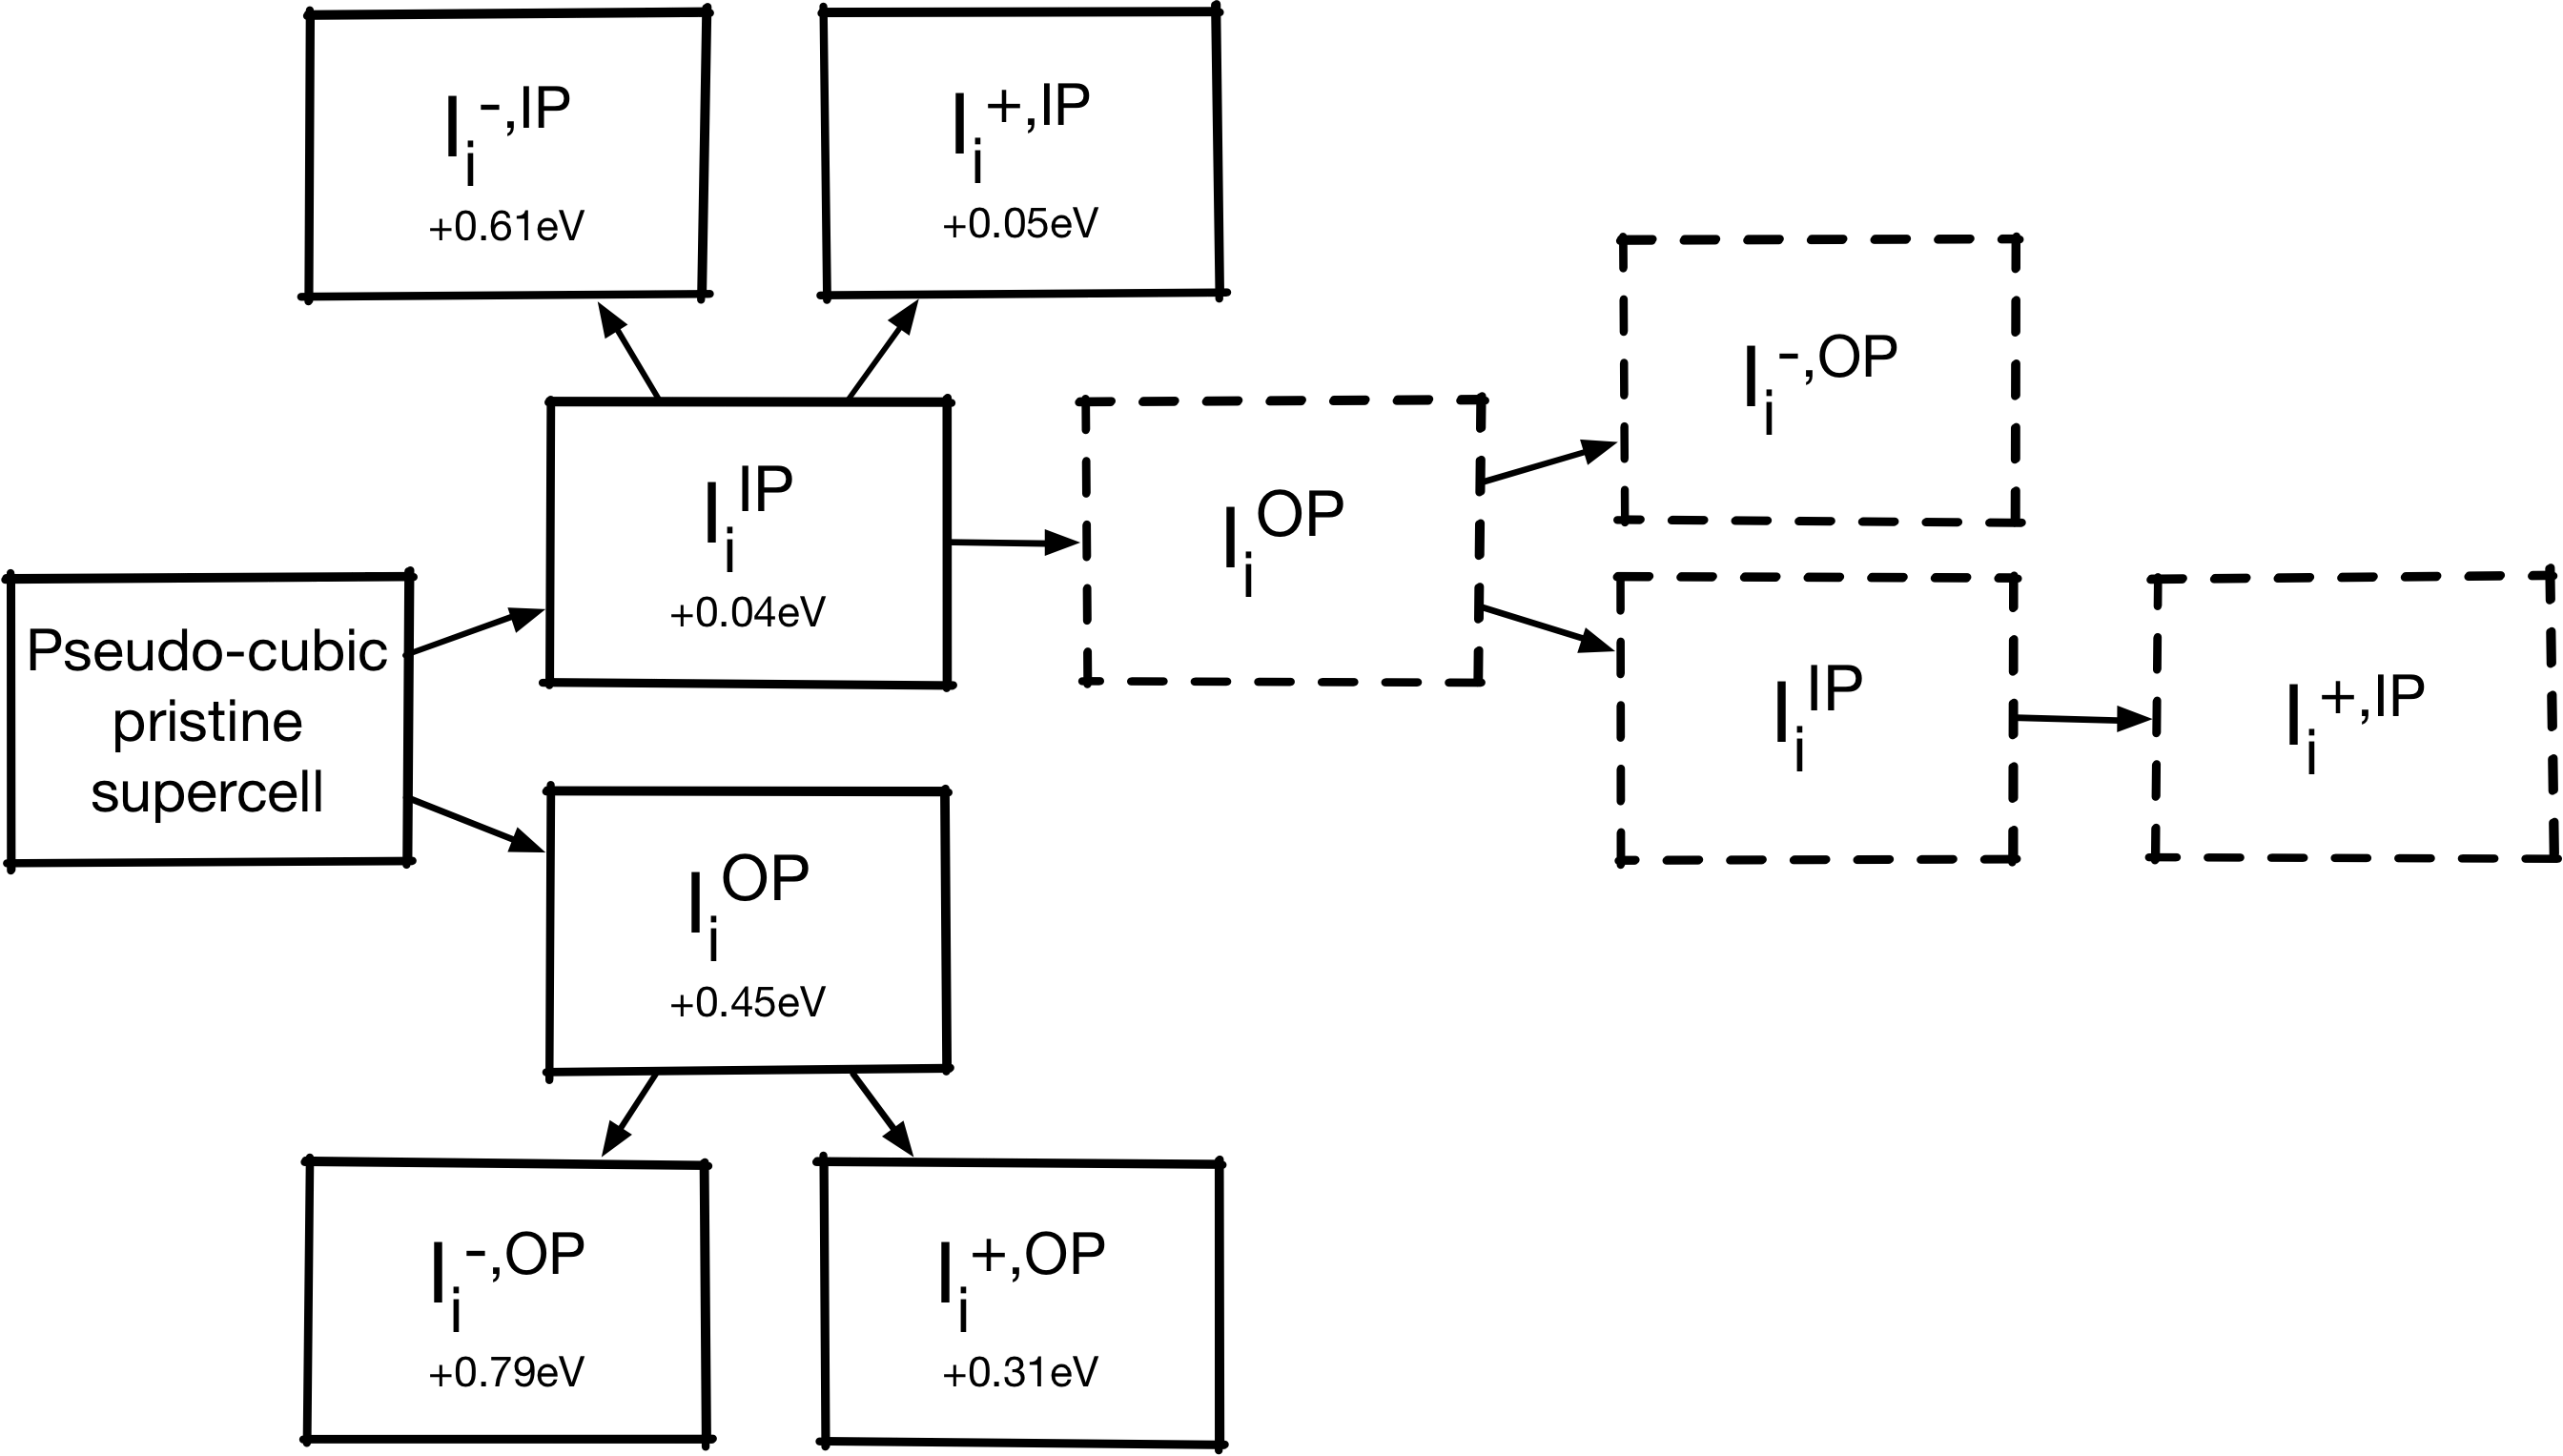
\includegraphics[width=0.7\columnwidth]{figures/ch6/relaxation_workflow.png}
  \caption[Atomic relaxation procedure for point defects in MAPI]{Atomic relaxation procedure for point defects in MAPI. Defect structures with the lowest energy for their charge state are in a dash-line box. The hybrid halide perovskite structure has a number of local minima and multiple relaxations were required to break symmetry and reach a global minimum. For the higher energy defect structures the energy above the global minimum for the relevant charge state is given.}
\label{relaxation_workflow}
\end{figure}

The neutral iodine interstitial $\mathrm{I}_\mathrm{i}$ relaxes to two defect geometries which differ by only \SI{0.04}{\electronvolt} in energy. The lowest energy structure contains a $\mathrm{I}_2^-$ split interstitial with bond length \SI{3.19}{\angstrom} lying out-of-plane along the $c$-axis. This is denoted $\mathrm{I}_\mathrm{i}^{\textrm{OP}}$. The higher energy structure contains a $I_2^-$ split interstitial with bond length \SI{3.24}{\angstrom} and lies in the $ab$-plane. This is denoted $\mathrm{I}_\mathrm{i}^{\textrm{IP}}$. The negative iodine interstitial 
$\mathrm{I}_\mathrm{i}^-$ relaxes to an out-of-plane position along the $c$-axis. It forms a split interstitial around an iodine lattice position with two independently coordinated iodide ions symmetrically bridging two lead atoms. The I--I distance is \SI{3.82}{\angstrom}. As $\mathrm{I}_\mathrm{i}^-$ lies out of plane, we expect potential charge trapping processes to occur between $\mathrm{I}_\mathrm{i}^-$ and $\mathrm{I}_\mathrm{i}^{\textrm{OP}}$. The positive interstitial forms an in-plane trimer structure with bond lengths \SI{2.89}{\angstrom} and \SI{2.95}{\angstrom}. As $\mathrm{I}_\mathrm{i}^+$ lies in-plane, we expect potential charge trapping processes to occur between $\mathrm{I}_\mathrm{i}^+$ and $\mathrm{I}_\mathrm{i}^{\textrm{IP}}$.
Table \ref{compare_geoms} contains a summary of the defect geometries alongside a comparison to values in the literature.

\begin{table}[h!]\centering
\begin{tabular}{llllllll}\toprule
\phantom{abcd}&\multicolumn{2}{c}{This work} &\phantom{a} &\multicolumn{2}{c}{Meggiolaro et al., Ref. \cite{Meggiolaro2018}}&\phantom{a} & Du, Ref. \cite{Du2015} \\
\cline{2-3} \cline{5-6} \cline{8-8}
& orientation & I--I bond length && orientation & I--I bond length && orientation \\  
\midrule
$\mathrm{I}_\mathrm{i}^-$ &  out-of-plane & 3.82  &&  out-of-plane & 3.89 && in-plane \\
$\mathrm{I}_\mathrm{i}^+$ & in-plane & 2.89/2.95 && in-plane & ave. 2.95 && in-plane \\
$\mathrm{I}_\mathrm{i}^\mathrm{OP}$ & out-of-plane & 3.19 && out-of-plane & 3.24 && - \\
$\mathrm{I}_\mathrm{i}^\mathrm{IP}$ & in-plane & 3.24 && in-plane & 3.88 && - \\
\end{tabular} 
\caption[Defect orientation and bond length of the $\mathrm{I}_\mathrm{i}^+$,$\mathrm{I}_\mathrm{i}^-$,$\mathrm{I}_\mathrm{i}^\mathrm{IP}$ and $\mathrm{I}_\mathrm{i}^\mathrm{OP}$ defects in MAPI]{Defect orientation and bond length of the $\mathrm{I}_\mathrm{i}^+$,$\mathrm{I}_\mathrm{i}^-$,$\mathrm{I}_\mathrm{i}^\mathrm{IP}$ and $\mathrm{I}_\mathrm{i}^\mathrm{OP}$ defects in MAPI, with a comparison to computational results in the literature. }
\end{table}

\begin{figure}[h!]
\centering
  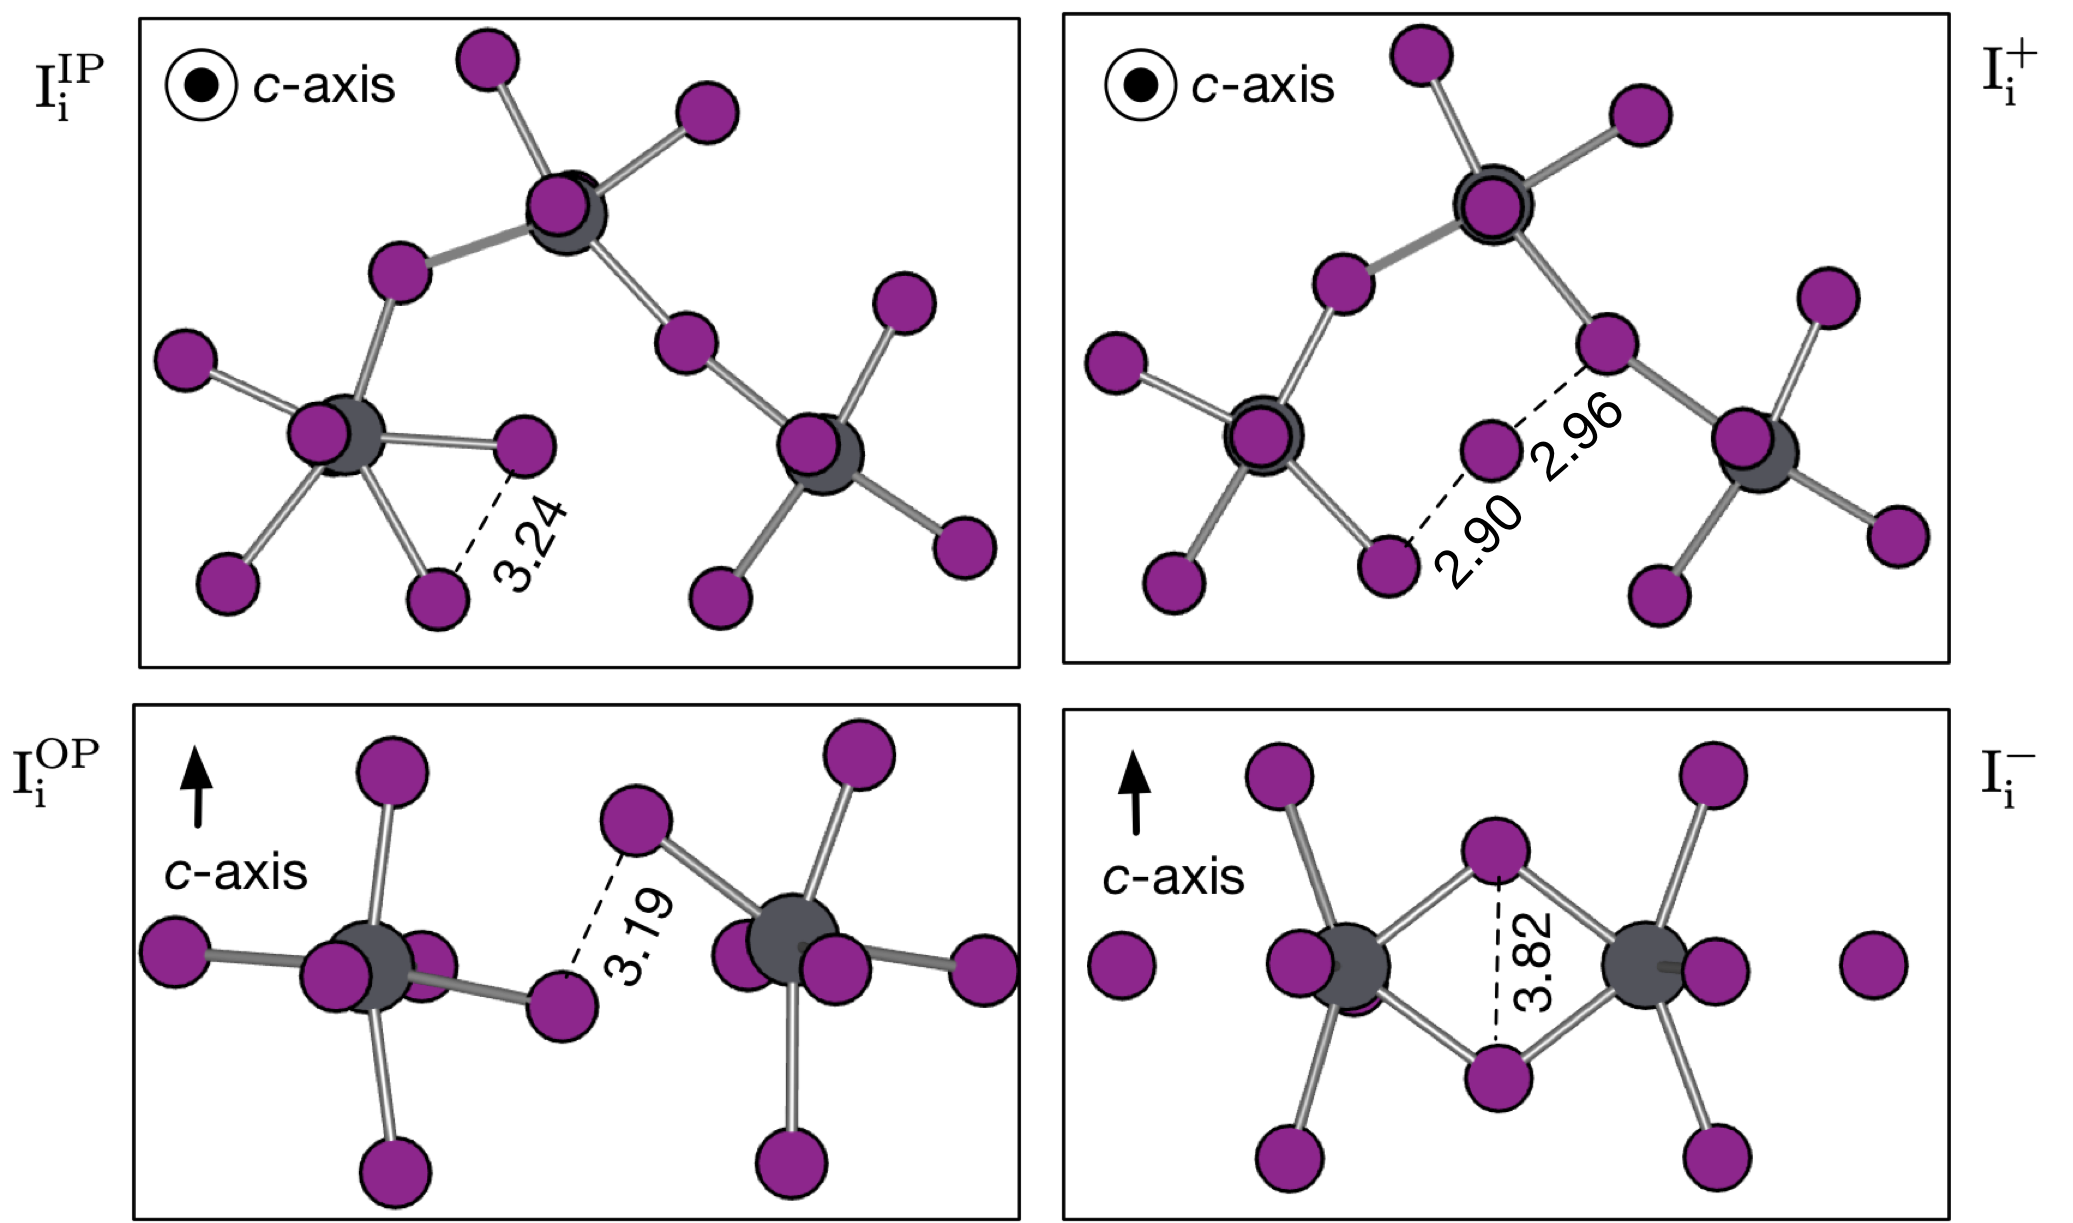
\includegraphics[width=1.0\columnwidth]{figures/ch6/defect_geometries.png}
  \caption[Defect geometries of the $\mathrm{I}_\mathrm{i}^+$,$\mathrm{I}_\mathrm{i}^-$,$\mathrm{I}_\mathrm{i}^\mathrm{IP}$ and $\mathrm{I}_\mathrm{i}^\mathrm{OP}$ defects in MAPI]{Defect geometries of the $\mathrm{I}_\mathrm{i}^+$,$\mathrm{I}_\mathrm{i}^-$,$\mathrm{I}_\mathrm{i}^\mathrm{IP}$ and $\mathrm{I}_\mathrm{i}^\mathrm{OP}$ defects in MAPI. IP indicates that the defect is lying in the $ab$-plane. OP indicates that the defect is lying along the $c$-axis.}
\label{relaxation_workflow}
\end{figure}

The I--I bond length in solid orthorhombic crystalline iodine is \SI{2.67}{\angstrom}, and the additional electron occupies an anti-bonding orbital..
% https://core.ac.uk/download/pdf/33330041.pdf . - trimer
% https://pubs.acs.org/doi/pdf/10.1021/j100265a035?rand=4xteqb9z - h-centre and neutral

%Structure of solid I2 is an orthorhombic zig-zag structure with intramolecular I–I bond lengths of 2.68 Å, and intermolecular I2 distances of 3.56 Å (ref. 24). This value of 2.68 Å can be considered as a primary covalent I–I bond and other forms of iodine chains where I2 donates to the σ* antibonding orbital in a charge transfer complex have significantly larger bond lengths23,25. For example, the triiodide ion, [I3]− in orthorhombic CsI3 has I–I bond lengths of 2.84 Å and 3.04 Å (ref. 26); one slightly higher than seen in covalent I2 and one longer bond possessing most of the additional charge. 

% discuss inequivalent iodine
% include displacement vectors, perhaps in appendix (mention script)

\subsection{Charge localisation} \label{ss:chglocal}
The spin-density plot in Figure \ref{} shows that the neutral iodine interstitial forms a spin-radical with a self-trapped hole.
The hole induces the formation of a bond between two iodine ions, producing a molecular dimer called a H-centre (Figure \ref{spin_localisation}). The formation of a H-centre is a well-established process, and has been studied in metal halide crystals since the 1950s.\autocite{} %CastnerKanzig
Whereas in the previous chapter we considered a large polaron, in this chapter we are studying a small polaron formed by the self trapped hole.
%quote schluger 1995 Kcl here also PRB doi: 10.1103/PhysRevB.52.4017 

\begin{figure}[h!]   %includes H-centre schematic
\centering
  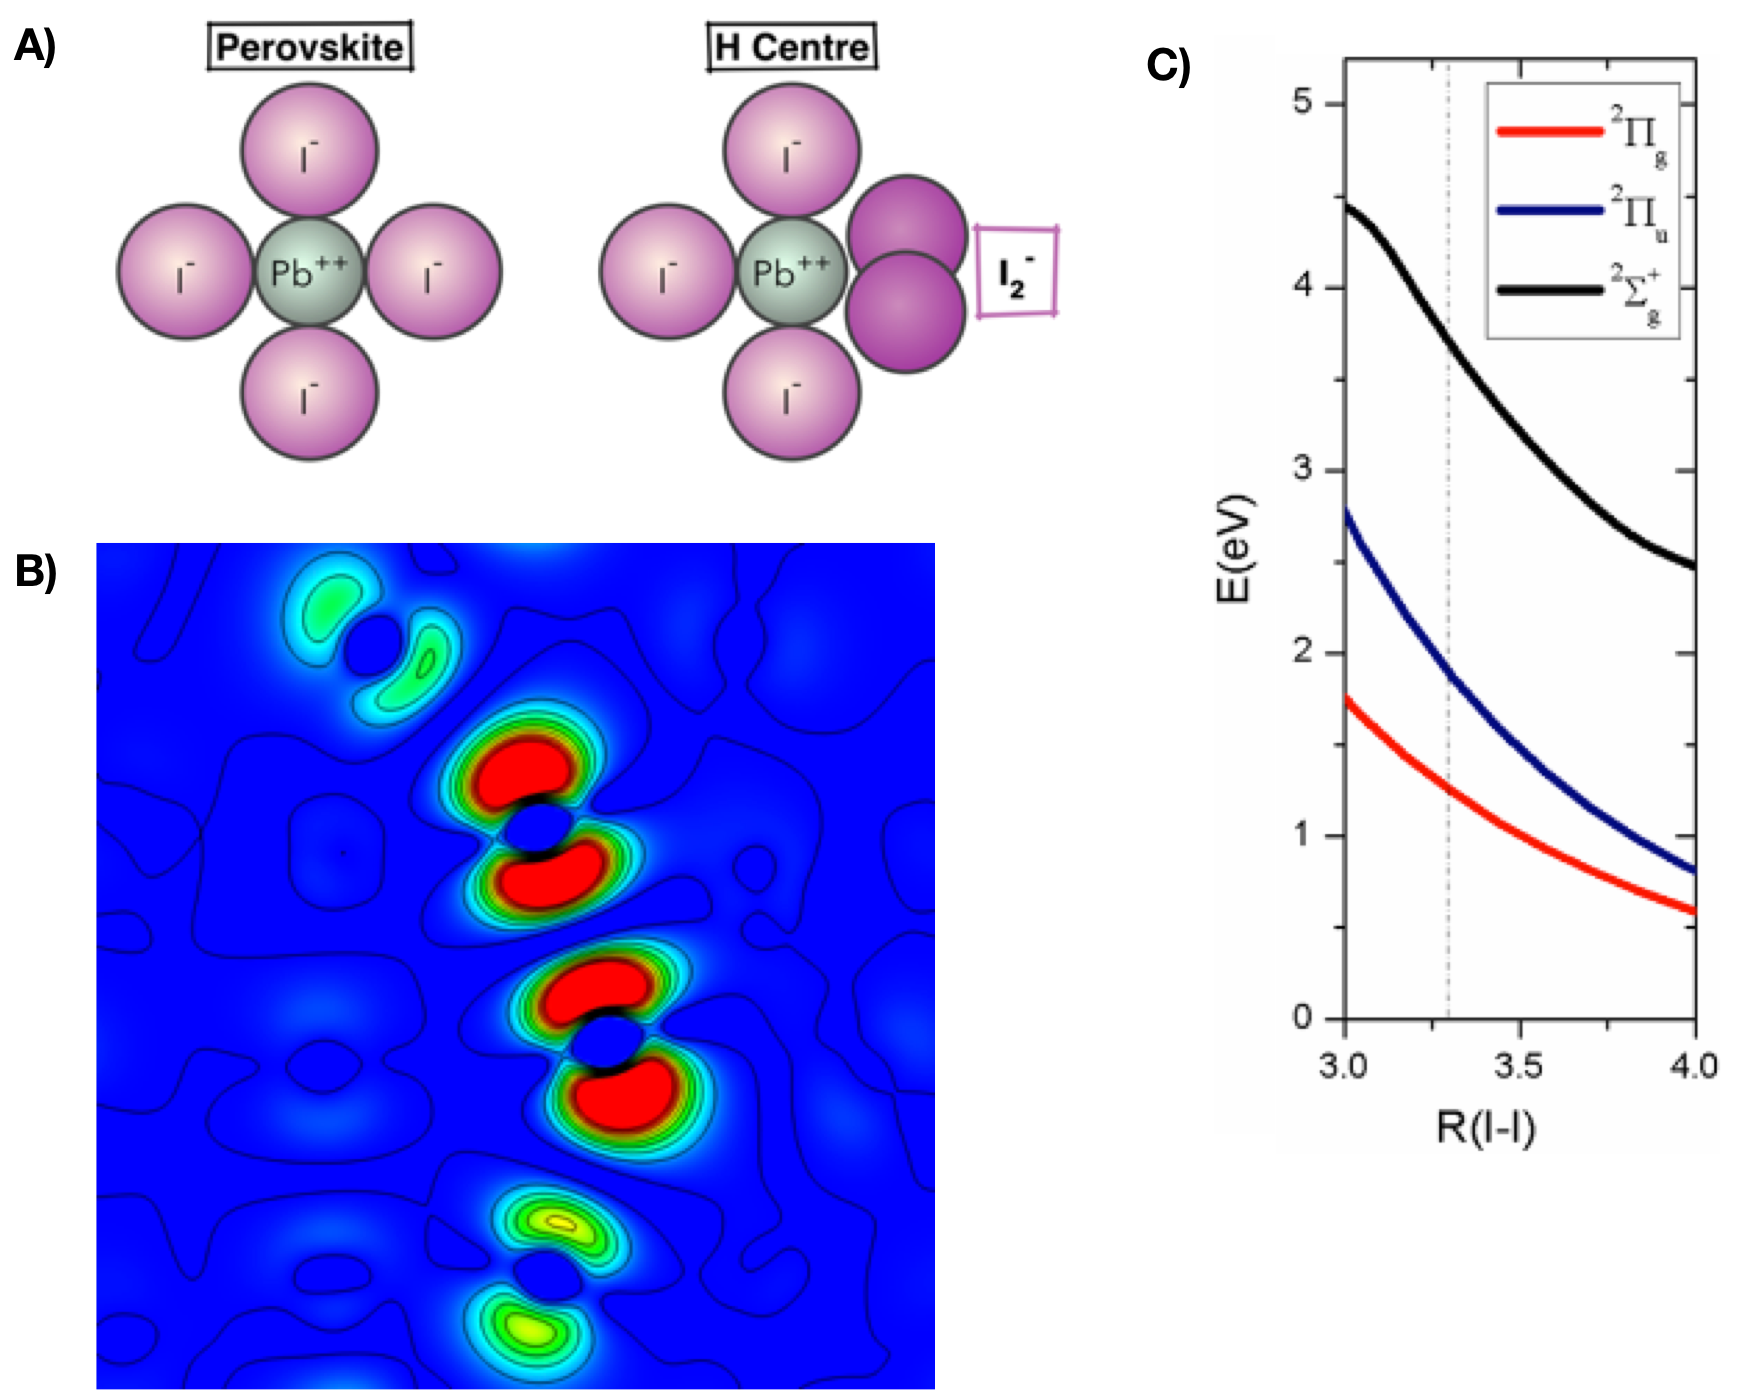
\includegraphics[width=0.9\columnwidth]{figures/ch6/spin_localisation.png}
  \caption[Spin localisation and optical excitation at the H-centre defect in MAPI]{A) Change in local equatorial environment around Pb in a lead halide perovskite upon formation of a H-centre defect. The H-centre is formed from a lattice iodide and interstitial iodide. The I--I interatomic spacing of ca. \SI{4.5}{\angstrom} in the perfect lattice decreases to a bond length of \SI{3.2}{\angstrom} upon dimer formation. Figure adapted with permission from an original prepared by Aron Walsh. B)  The difference between the density of the two spin channels in a spin-polarised calculation is plotted to show spin localisation around the H-centre defect in MAPI. C) Optical excitation energies as a function of dimer bond length for the iodine dimer in MAPI.}
\label{spin_localisation}
\end{figure}

The H-centre is a ``molecule-in-a-crystal'' defect where the host weakly perturbs the $I_2^-$ molecular ion.
This allows consideration of the optically excited states using a dielectric embedding approach.\autocite 
A collaborator, Rachel Crespo-Otero, has computed the optically excited states of the H-centre defect as a function of bond lengths using time-dependent DFT including relativistic effects (see Figure \ref{optical_excitation}).
For the bond lengths found in the MAPI host (\SI{3.19}{\angstrom}), the three lowest excited states occur at \SI{}{\electronvolt} (symmetry-allowed), \SI{}{\electronvolt} (forbidden), and \SI{}{\electronvolt} (symmetry-allowed). Two optically allowed transitions fall in the visible−ultraviolet range, and a sub-band gap absorption band at ca. \SI{}{\electronvolts} should be observable in long-wavelength absorption measurements if present in sufficient concentration.

\subsection{Defect formation energies} \label{ss:dfe}

The formation energy of a defect in charge state $q$ is given by

\begin{equation} \label{eqn_formation_energy}
E_\mathrm{f}(q) = E_\mathrm{d}(q) - E_\mathrm{b} - \sum_i \mu_i n_i + q(\epsilon_\mathrm{VBM}+E_\mathrm{F}) + E_\mathrm{corr}.
\end{equation}
The total energy of the supercell $E_\mathrm{d}(q)$, the total energy of the pristine lattice $E_\mathrm{b}$ and the iodine chemical potential $\mu_i$ were calculated DFT as outlined in the methods section.
The defect correction $E_\mathrm{corr}$ consists of two terms - the charged defect correction and a `tilting' correction that is specific to pseudocubic perovskites.
Both terms are small. The charged defect correction is equal to \SI{X}{eV}. This is due to the high dielectric constant of MAPI (, from Ref. []) that allows effective ionic screening of charged defects. The point defects themselves have a maximum charge of one which also leads to small charged defect corrections.
The tilting correction is a new correction introduced in this work and particular to pseudocubic perovskites. All of the defect formation energies are referenced to a pristine lattice energy. The pristine lattice in the pseudocubic phase corresponds to a time average and is not the minimum energy structure.
% tilting correction results: 
    %We expect the tilting correction to scale linearly with supercell size
    %See work published in Ruoxi's thesis
    %270/37 = 7.5 ~ 8 which is to be expected as supercell is 8* bigger
    %We expect reduction of 2*37meV for 192 supercell = 0.074eV
     % Schematic of what is happening Although small, important as exponential term.


% negative U characteristic of previous work
% however two charge states
%app:7-chargetransition - in line with previuos and shows senstivitiy
% negative formatin enrgies - how cna be improved



% negative U behaviour
% two electron nature: no trapping

\begin{figure}[h!]   
\centering
  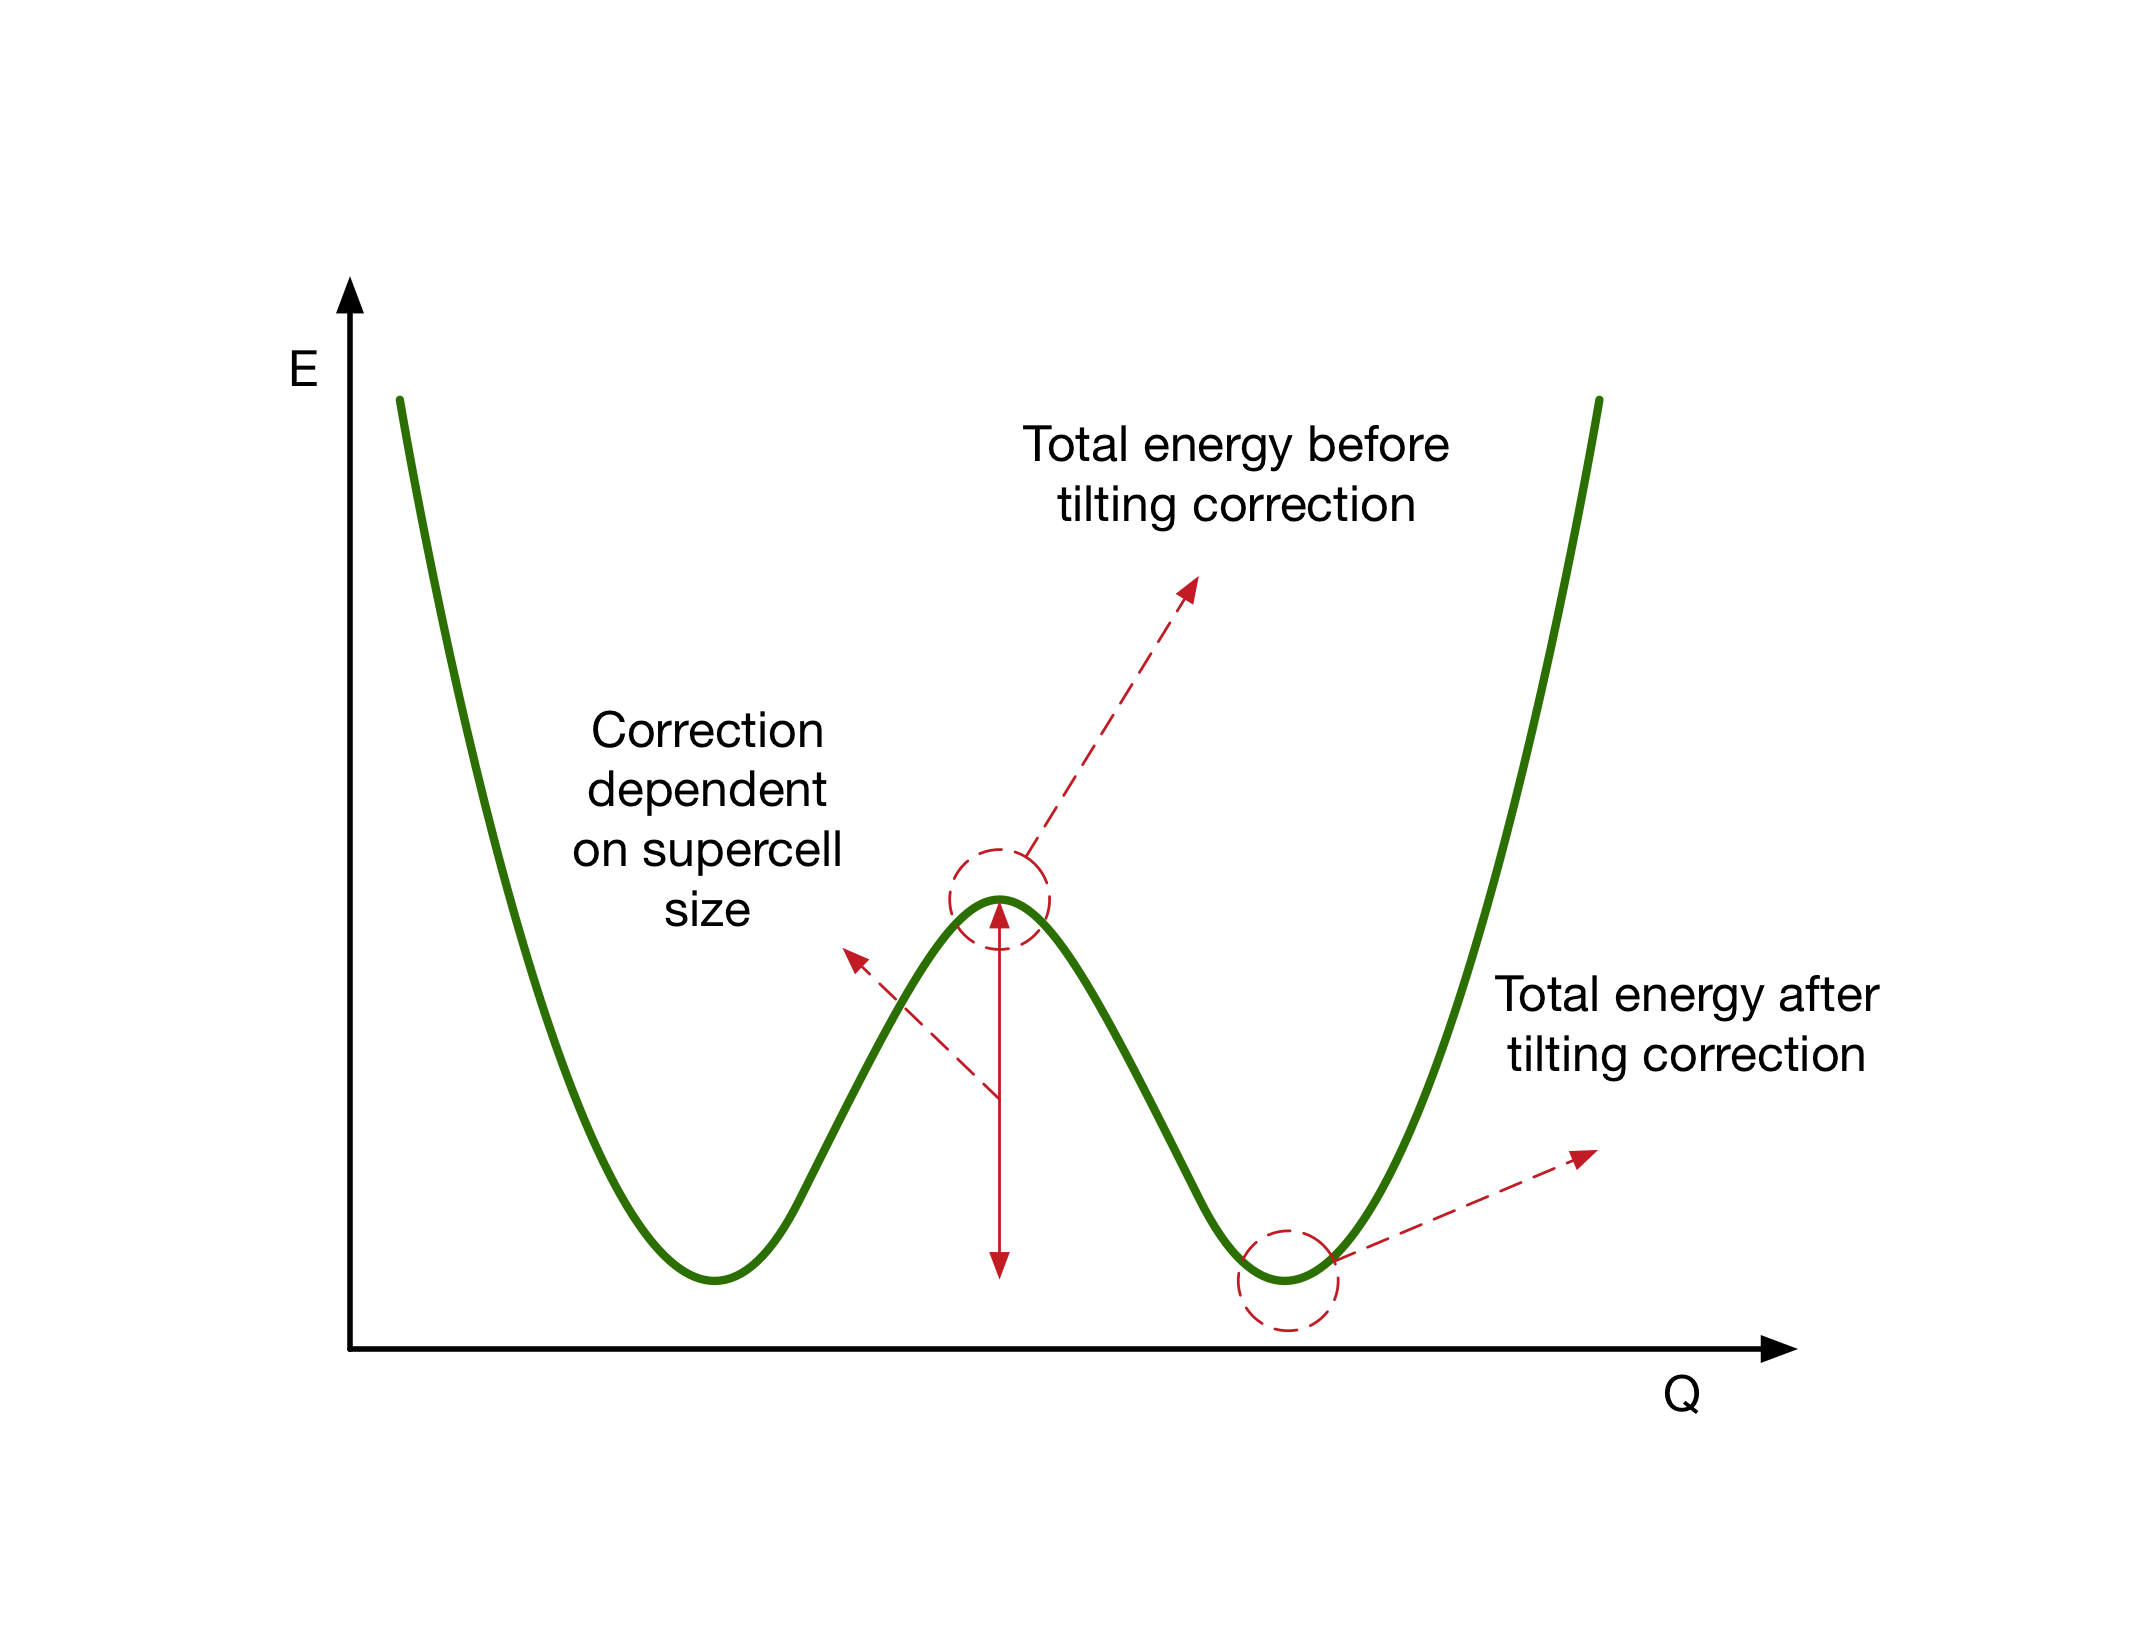
\includegraphics[width=0.7\columnwidth]{figures/ch6/tilting_correction.png}
  \caption[Tilting correction for defect formation energies]{An outline of the tilting correction for defect formation energies.}
\label{tilting_correction}
\end{figure}

\begin{figure}[h!]   
\centering
  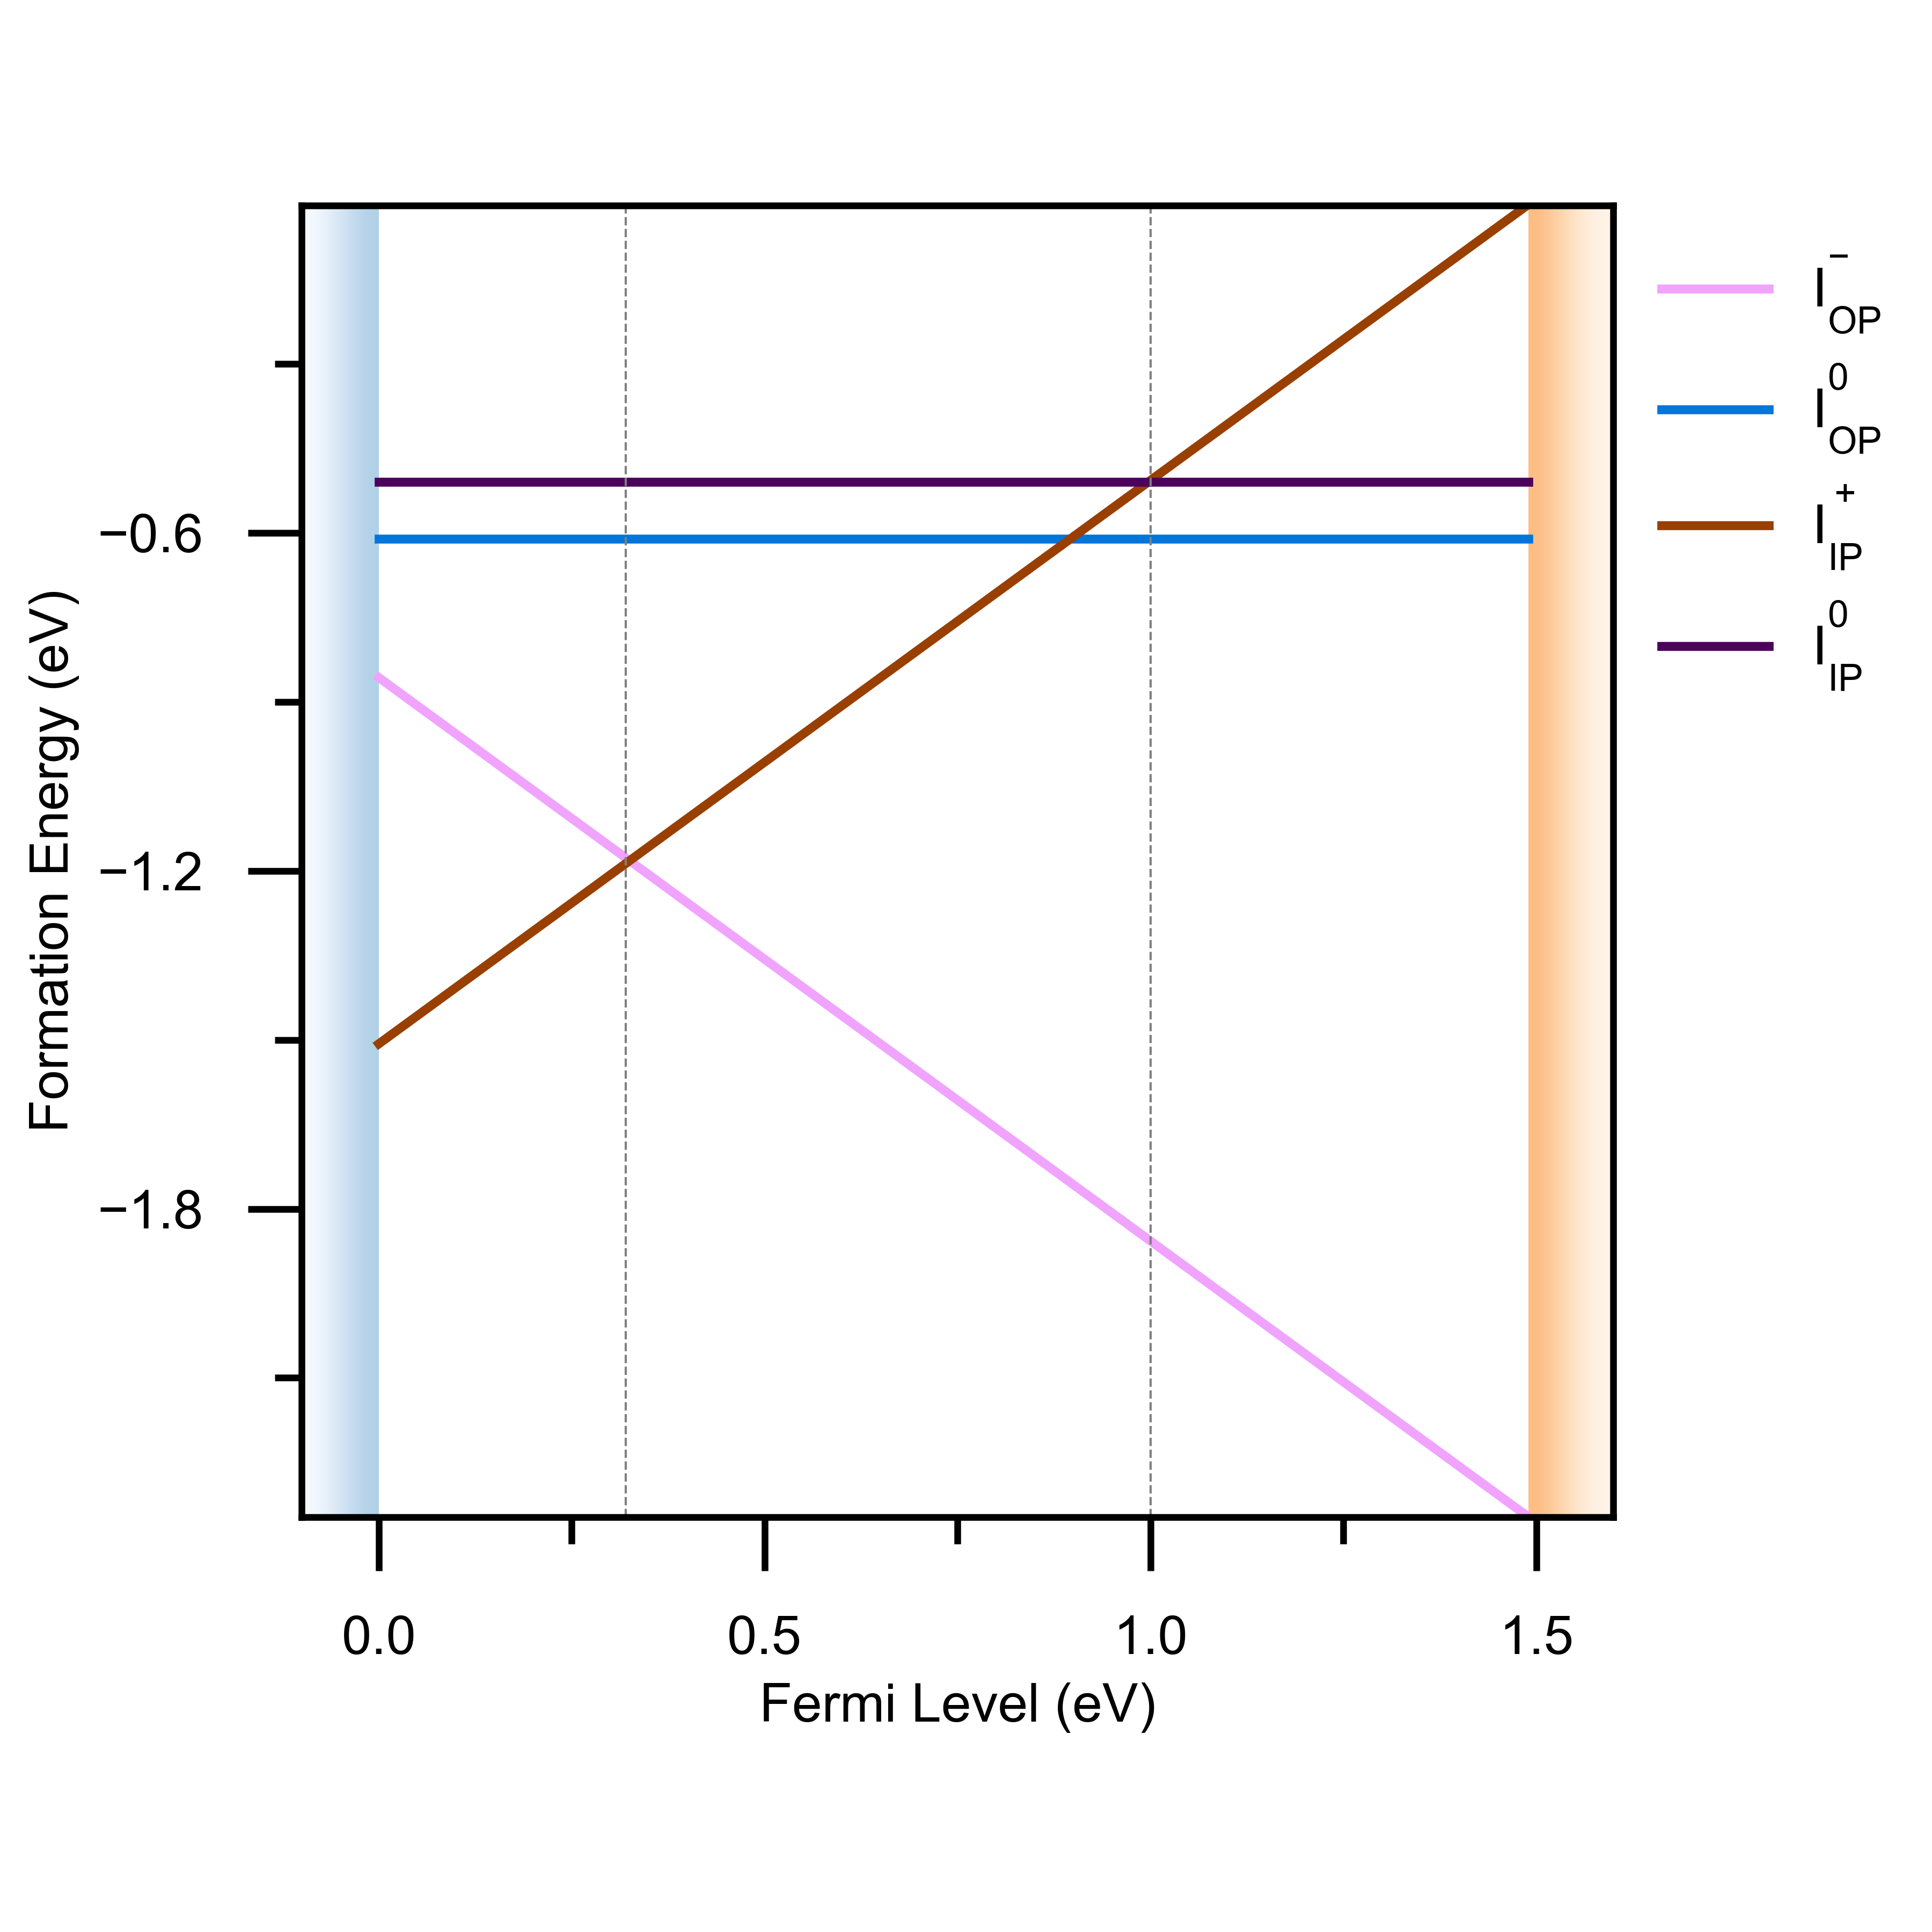
\includegraphics[width=0.7\columnwidth]{figures/ch6/charge_transition_HSE.png}
  \caption[Charge transition diagram for the iodine interstitial defect in MAPI]{Charge transition diagram for the iodine interstitial defect in MAPI.}
\label{charge_transition_diagram}
\end{figure}
% need to update defect notation!



\subsection{Configuration Coordinate diagram}

Collective coordinate Q like previous

 The physical  basis of this model for the description of the optical properties of localized centres in solids has been well documented [l01 and is based on the adiabatic Born-Oppenheimer approximation.  The  model assu- mes that the  electronic states  of the centre  interact appreciably with only one normal mode of the lattice Q, and that in the electronic ground state the equilibrium position of the ions is  Q = 0. In the excited electronic state the equilibrium position  is at Q = A, and in general the shape of the potential energy curve differs from that for the ground  state. Both curves are assu- med to be  parabolae i. e.  the vibrations are harmonic. The scheme is  shown in figure 1
 
 % Plot of the schrodinger solution is in the appendix.
 
 
\begin{figure}[h!]   
\centering
  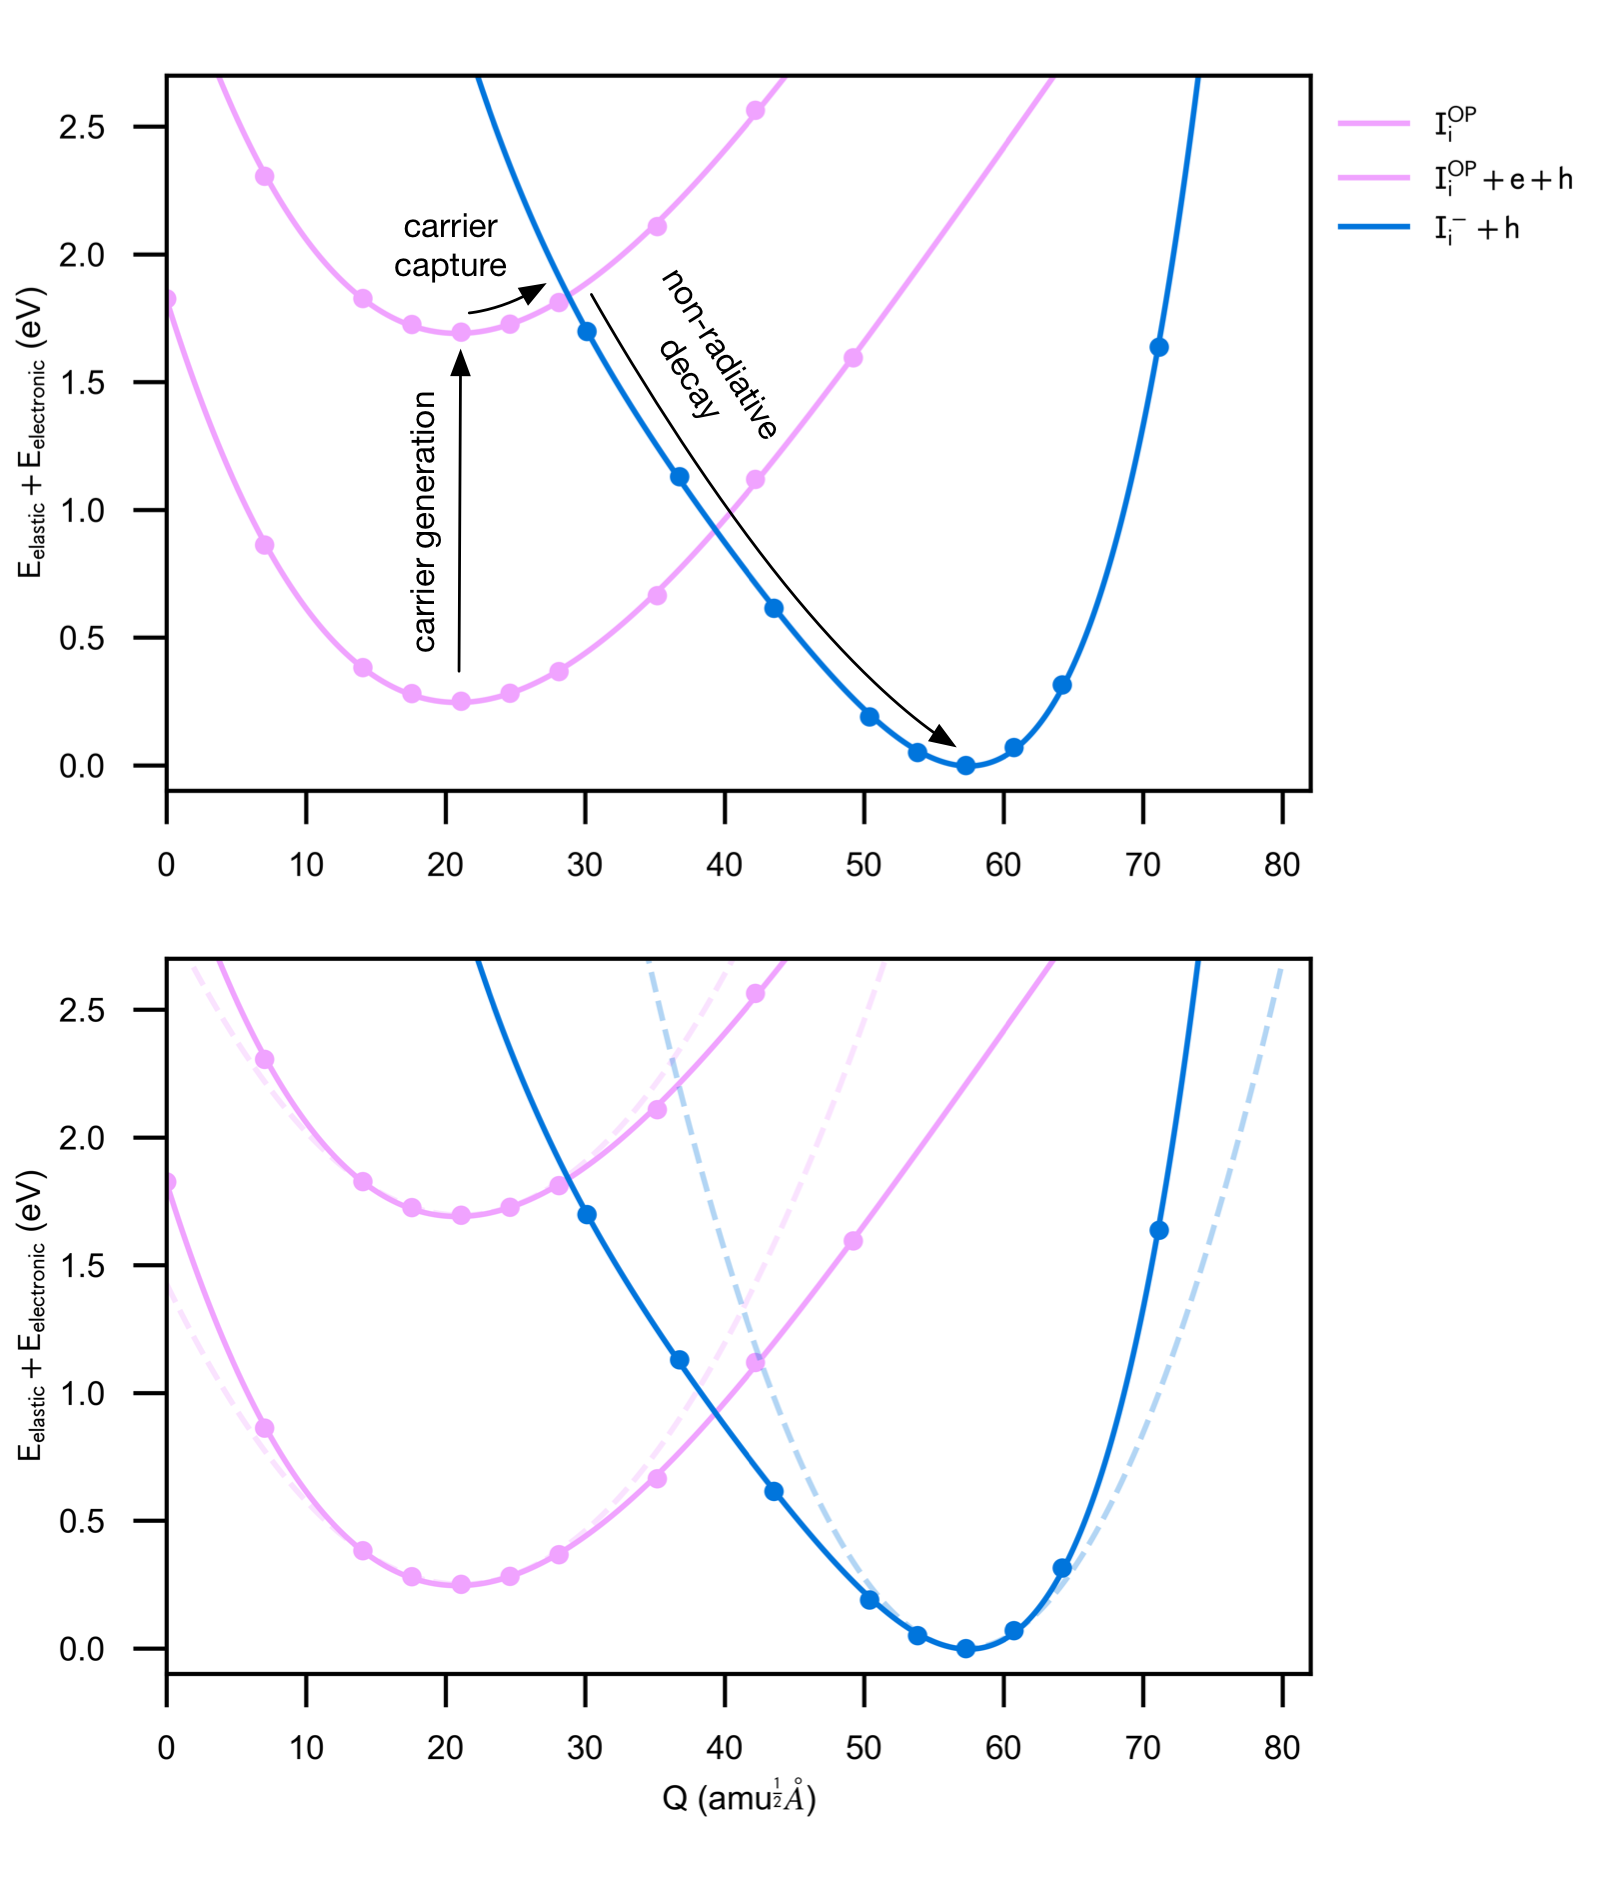
\includegraphics[width=1.0\columnwidth]{figures/ch6/carrier_capture_digram.png}
  \caption[Configuration coordinate diagram for carrier capture between negative and neutral charge states of the iodine interstitial defect]{Configuration coordinate diagram for carrier capture between negative and neutral charge states of the iodine interstitial defect}
\label{configuration_coordinate}
\end{figure}

% talk about the need to distort along the inorganic only

 % Calculate S and comment: https://hal.archives-ouvertes.fr/jpa-00213295/document

% include significance of large distortion: it is small if measured one way, large if measured another way. But its actually huge! Significance of this.
% for lovely discussion see Alkauskas:
% https://www.osti.gov/pages/servlets/purl/1471061
%"It might be surprising that this one-dimensional approximation to what is
%essentially a multi-dimensional problem (where the dimensionality is 3N, N being the number of atoms in the system) is
%sufficient. The beauty of 1D cc diagrams is that often they are
%sufficient.51 As discussed in the Appendix, this is particularly the
%case for defects with strong electron–phonon coupling. In certain
%cases, the validity of this approximation can be demonstrated rigorously; we discuss one such example in the Appendix."

% Need to make CC diagram. 
% All the CC diagrams should be referenced to zero.
% use linear interpolation
% interpert CC
% CC diagram with schrodinger solution superimposed.
% problem with the adiabatic approach and falling to the local minima
% talk ahout the difference between the photochemistry and equilibrium thermodynamics
% calculate the harmonic PES to show why the anharmonic is important

%that the CC diagram is incredibly soft and the equivalent harmonic frequency

% Appendix with additional configuration coordinate diagrams:
% - at different levels of theory.

\subsection{Vibrational properties}

In the previous section the coupling of a  defect to lattice vibrational modes was discussed without particular reference to the types of mode involved. The normal modes of a crystal containing a  defect may be  divided into three kinds : lattice modes, pseudo-localized or resonant modes, and localized modes. The lattice modes approximate closely to the normal modes of the perfect crystal, and have the same amplitude  throughout the whole crystal, except near the defect where there may be some small modifi- cation. On the other hand the resonant modes, although not strictly localized since their frequencies lie within the continuum of lattice modes, have a high amplitude near the defect and even a small number or density of resonant modes can give an appreciable contribution to the vibrational structure observed. 
% including IPR
% Emphasise that the agreement between IPR and configuration coordinate shows that the approximation of a 1D PES is great in this instance.
%upload on Youtube
% include Julia phonons work! distortion projected 

\begin{figure}[h!]   
\centering
  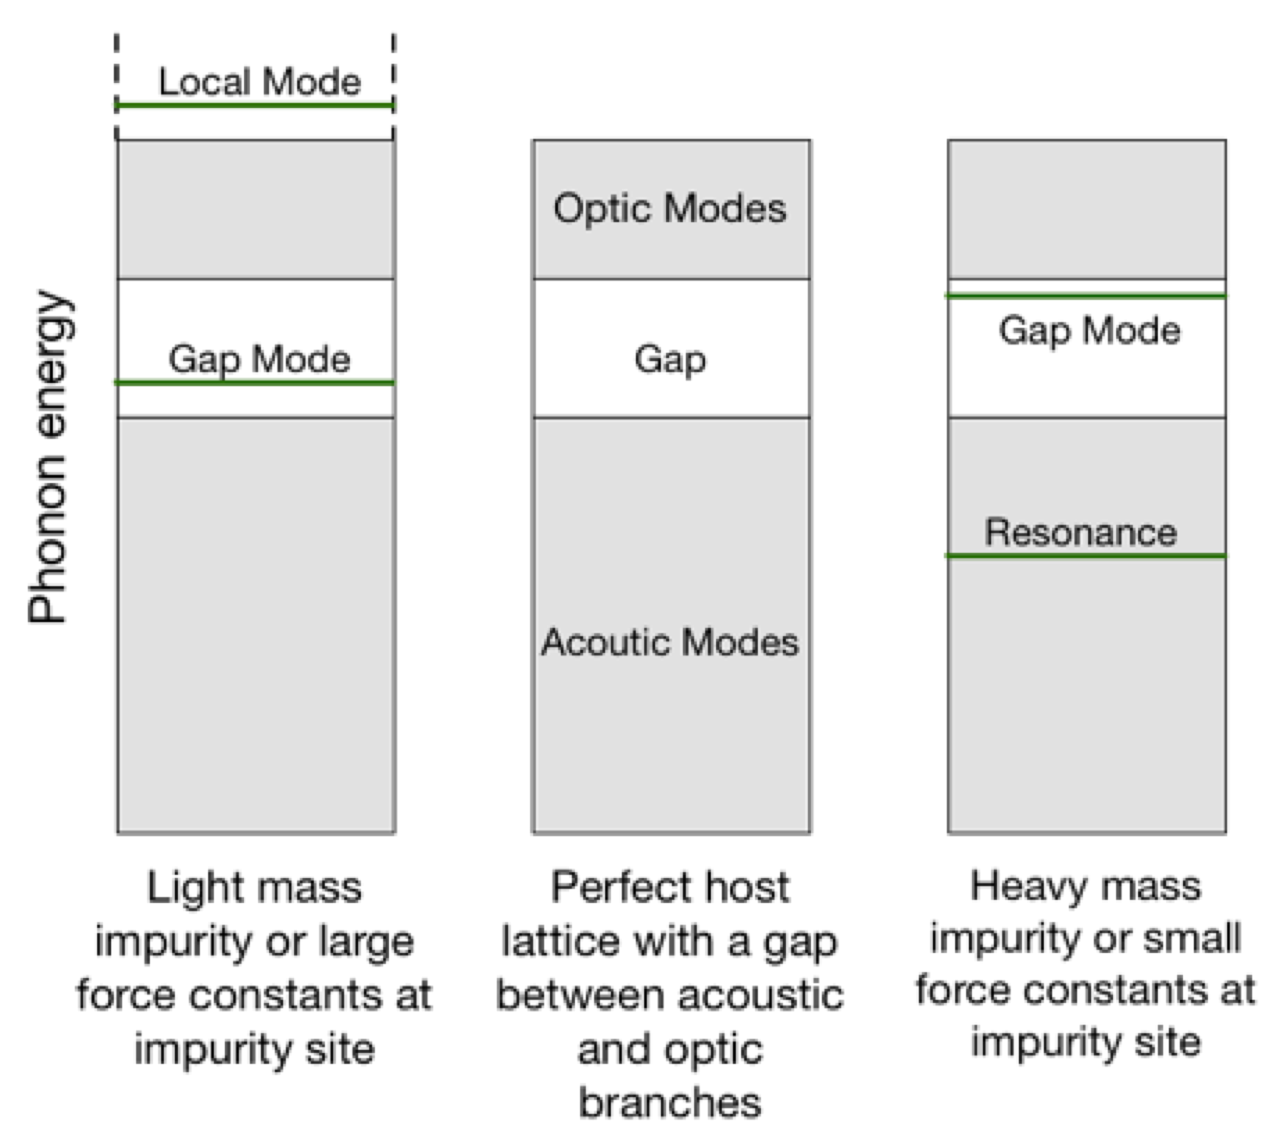
\includegraphics[width=0.6\columnwidth]{figures/ch6/defect_modes_schematic.png}
  \caption[The three kinds of mode found in a crystal with a defect]{}
\label{defect_modes_schematic}
\end{figure}

\begin{figure}[h!]   
\centering
  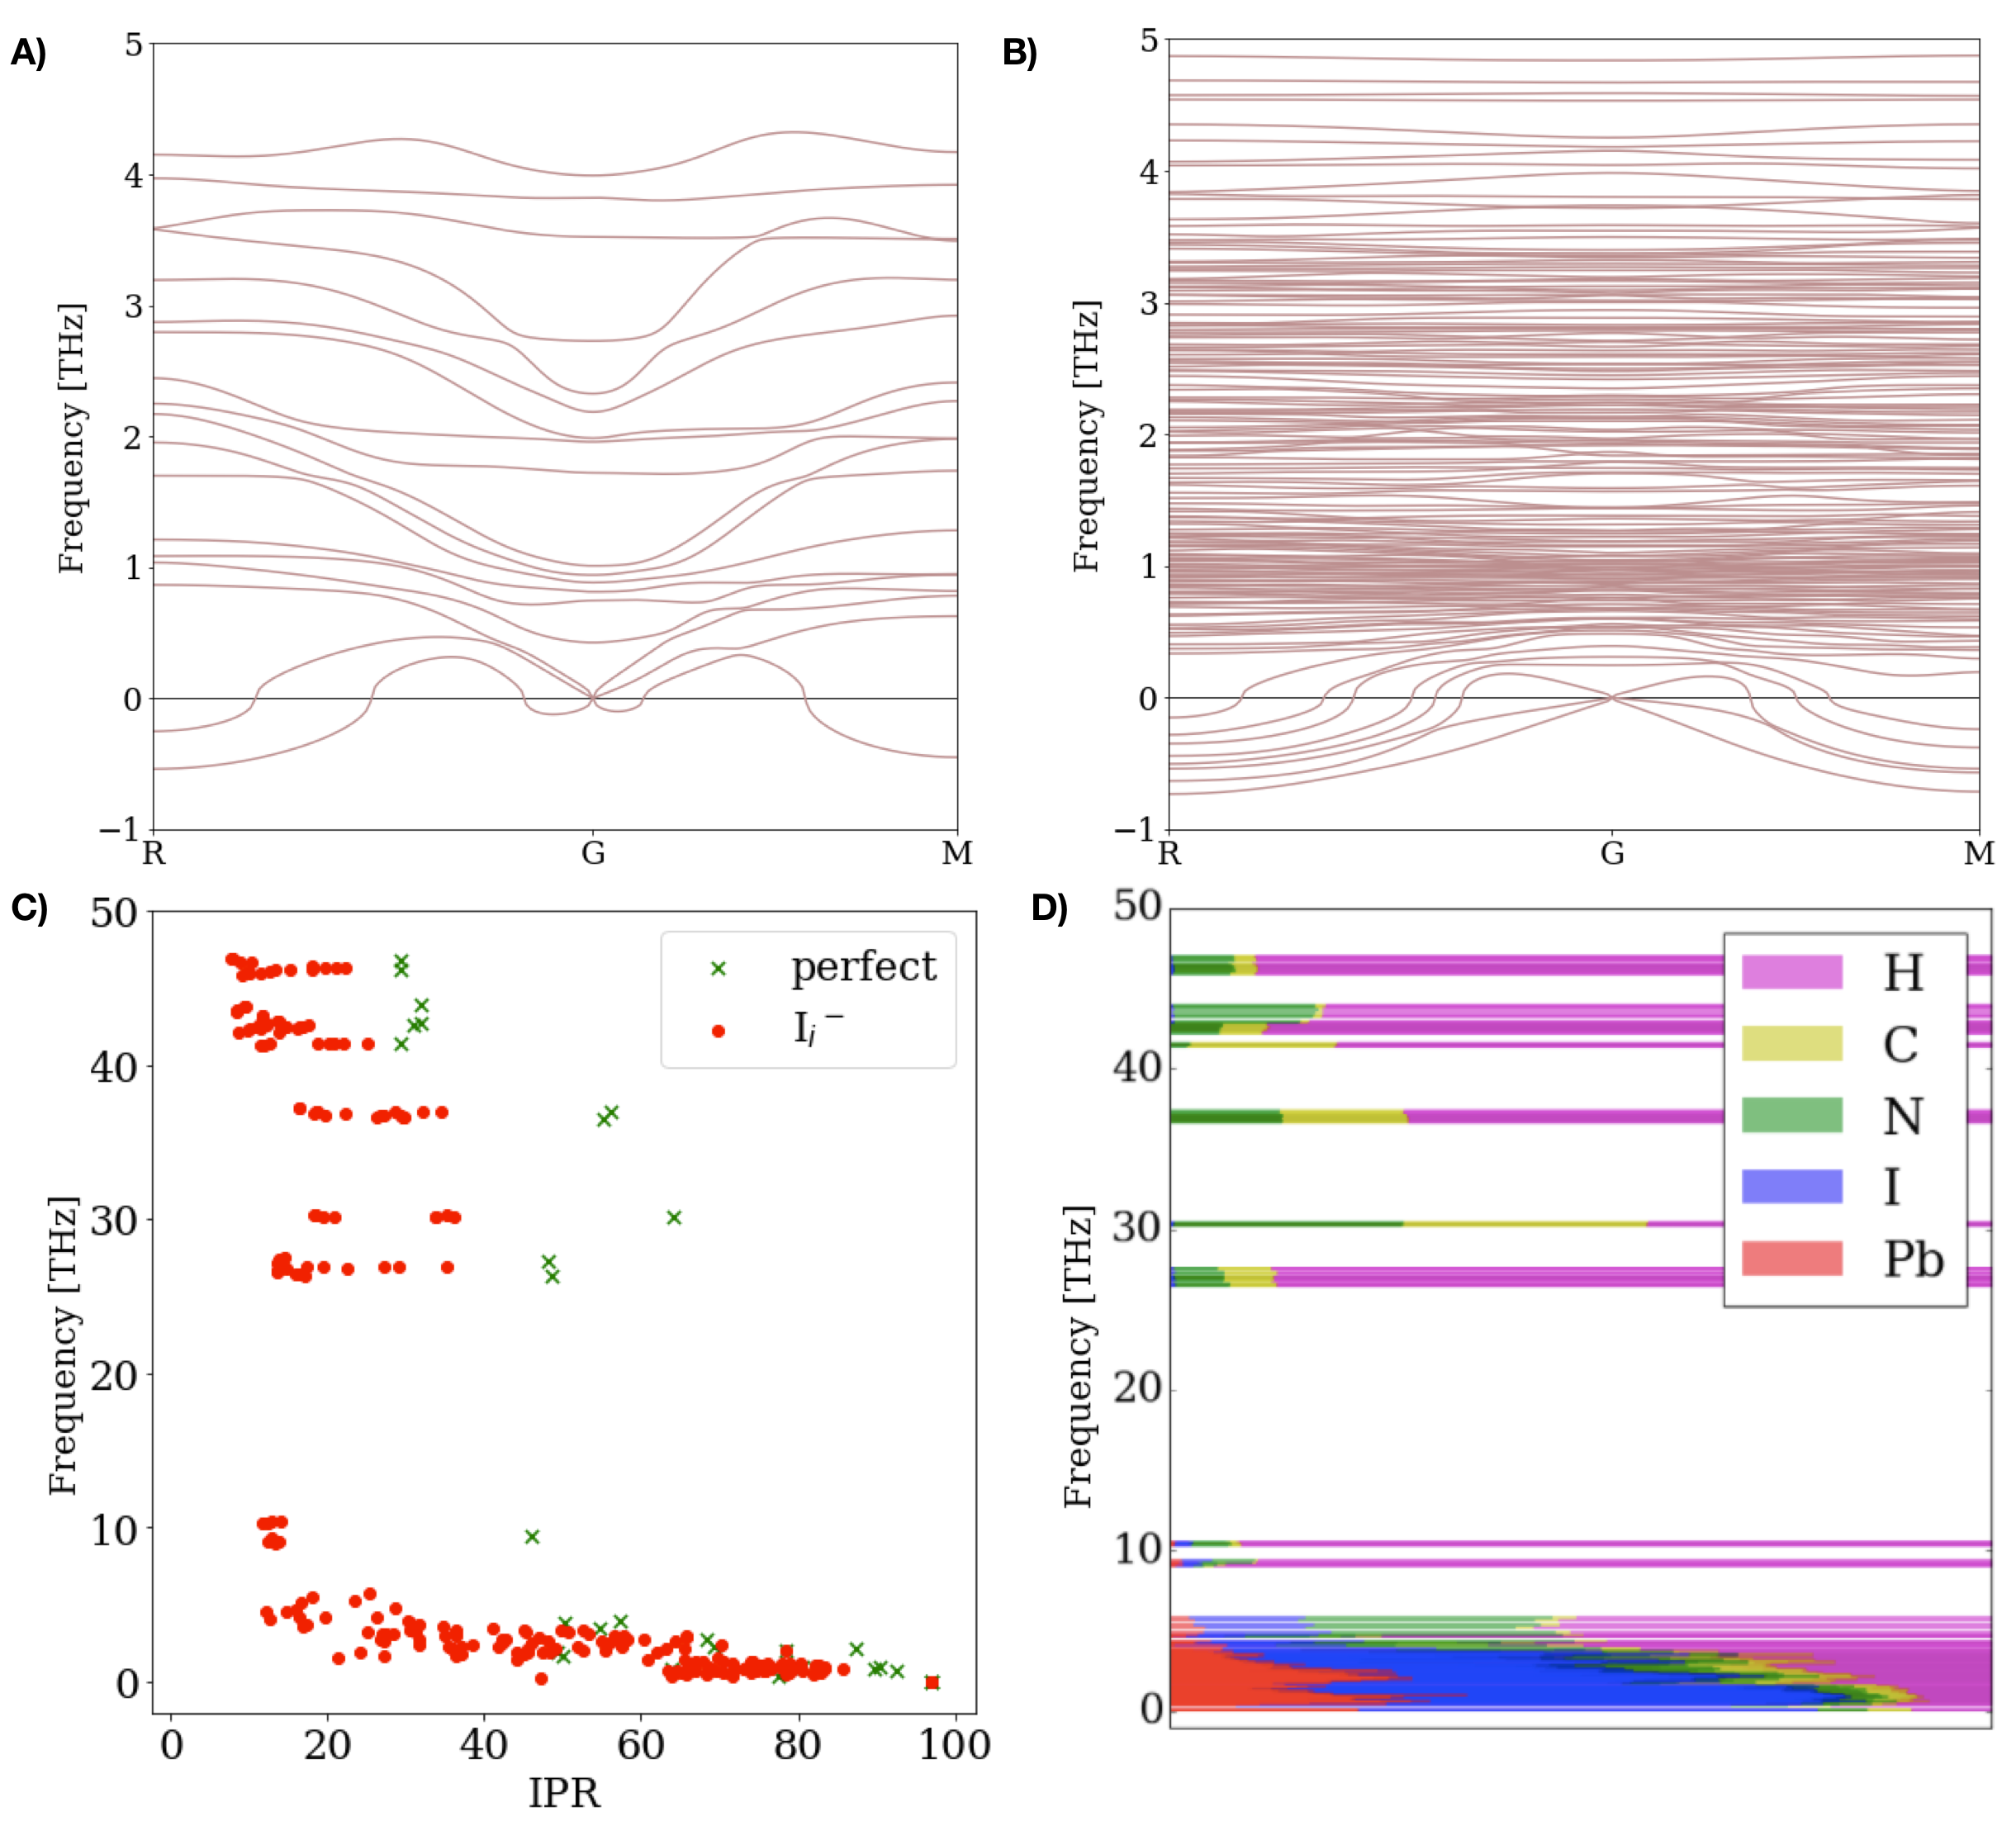
\includegraphics[width=1.0\columnwidth]{figures/ch6/defect_dispersion_IPR.png}
  \caption[Phonon dispersion and Inverse Participation Ratio of a MAPI crystal containing $\mathbf{I}_i^{-}$]{Phonon dispersion and Inverse Participation Ratio of a MAPI crystal containing $\mathbf{I}_i^{-}$}
\label{defect_dispersion_IPR}
\end{figure}


\subsection{Carrier capture mechanism and rate}


\begin{figure}[h!]   
\centering
  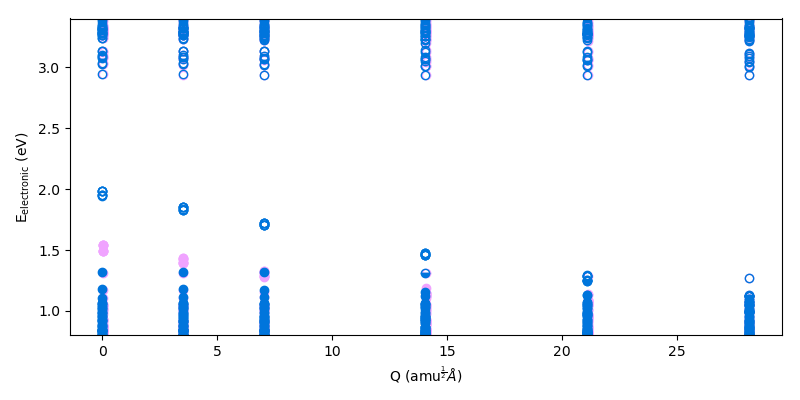
\includegraphics[width=1.0\columnwidth]{figures/ch6/eigs.png}
  \caption[ ]{}
\label{eigenvalues}
\end{figure}


\begin{figure}[h!]   
\centering
  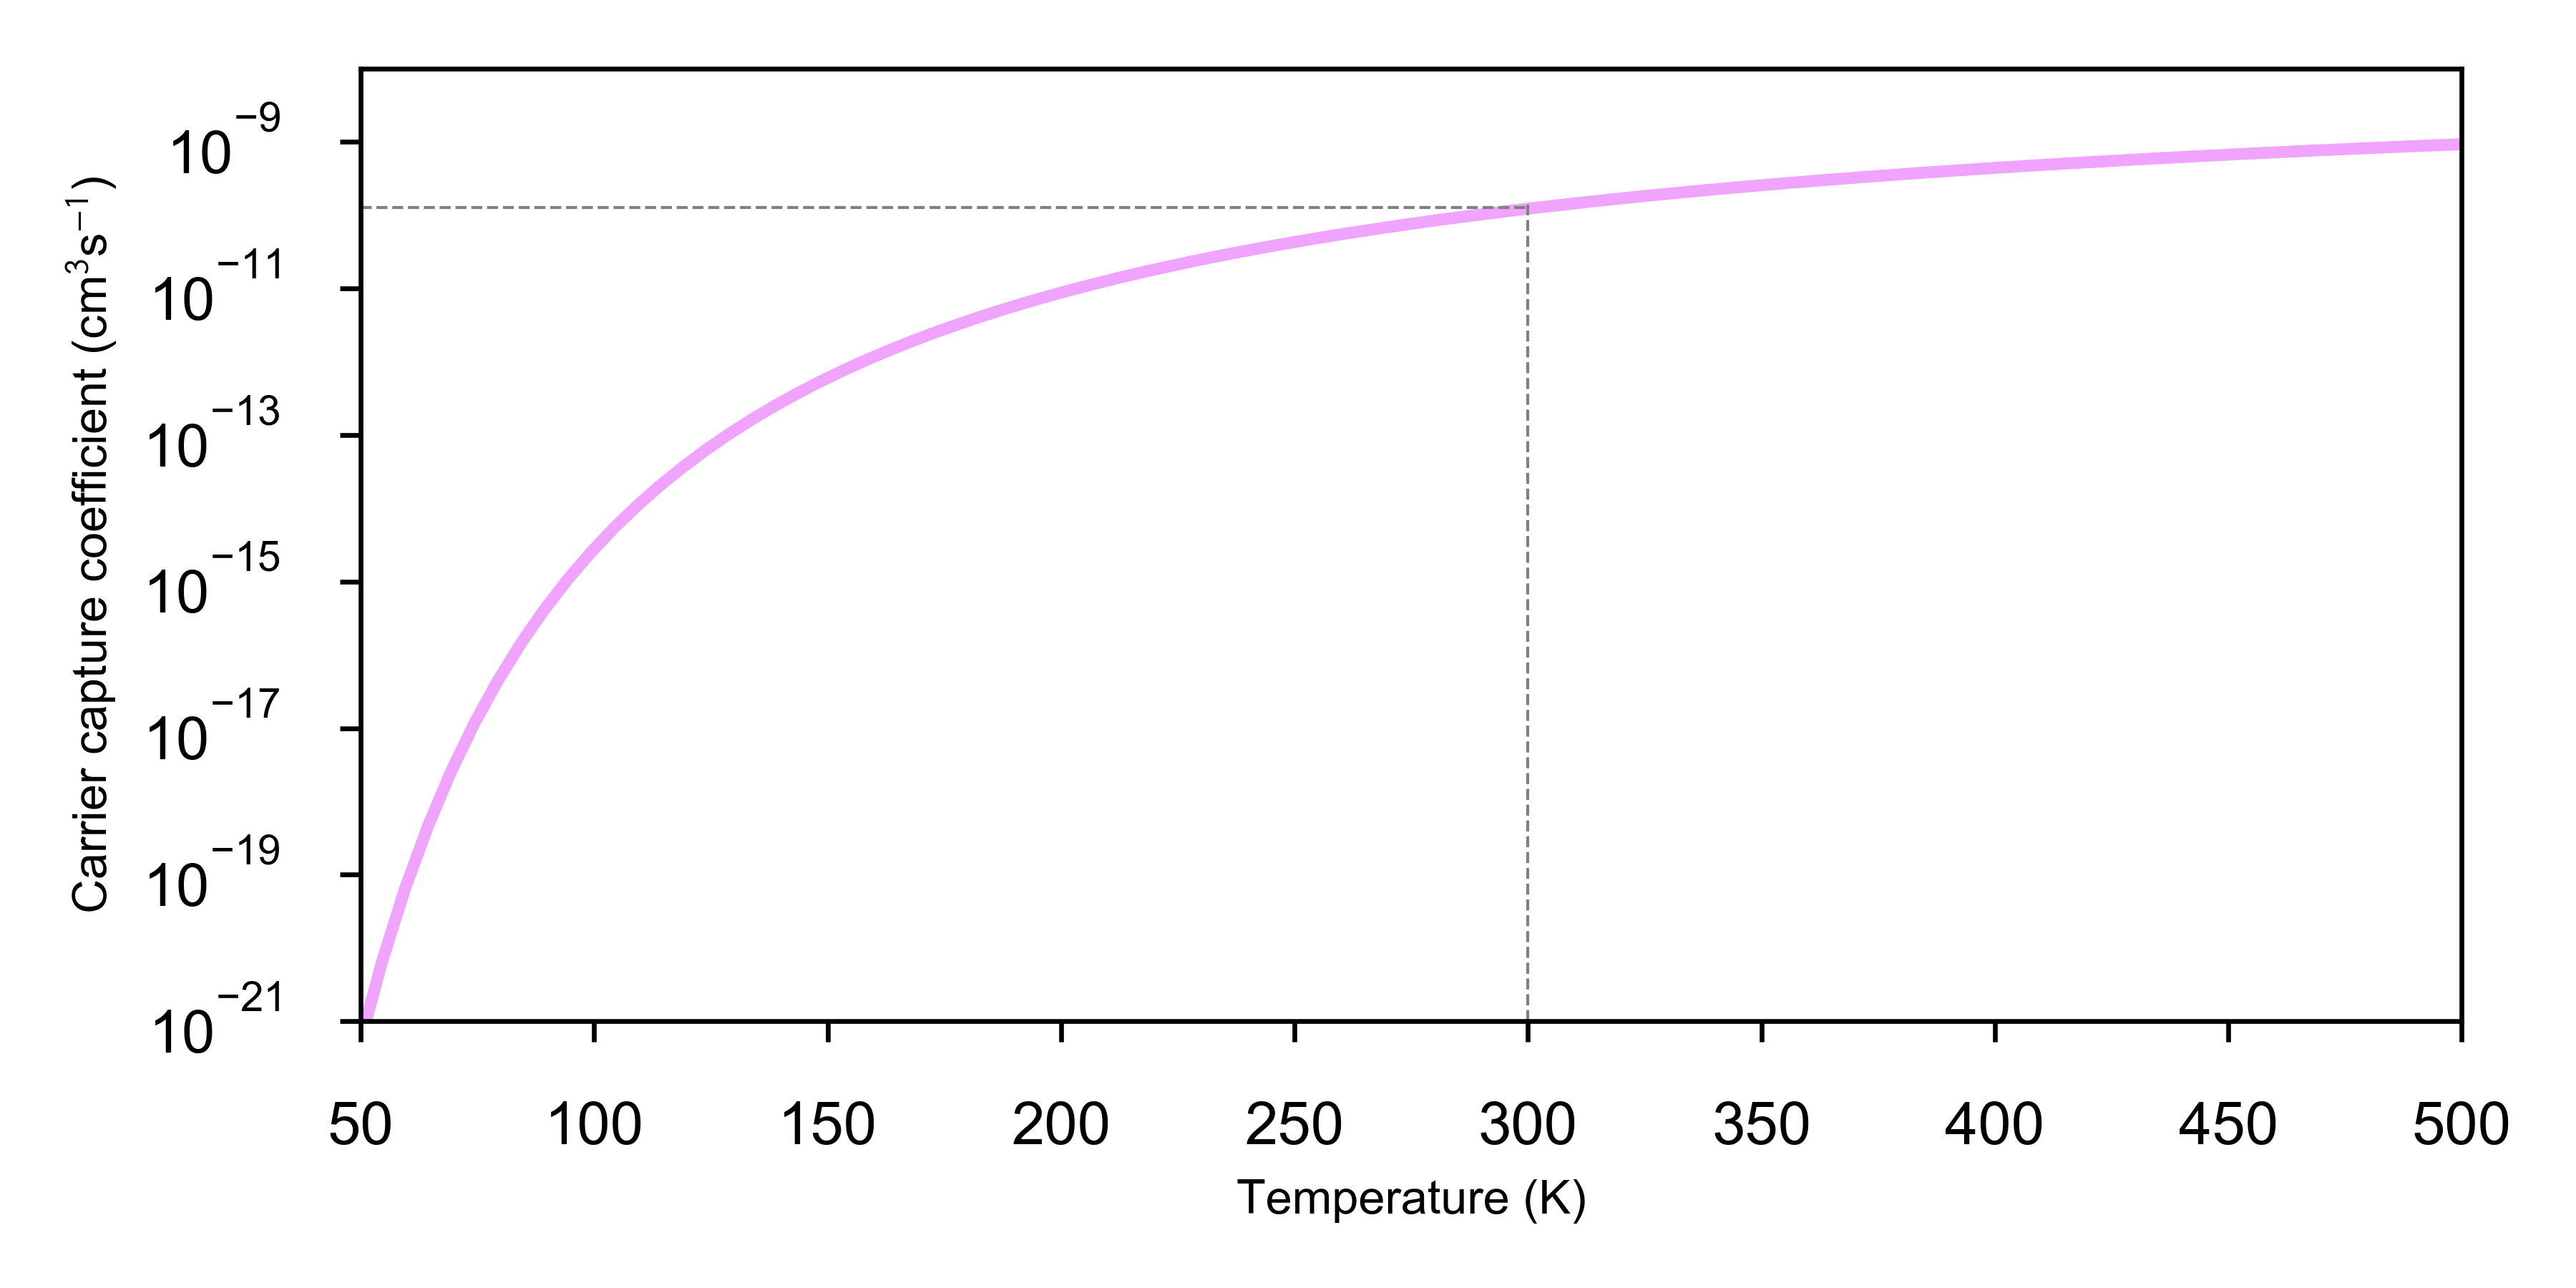
\includegraphics[width=1.0\columnwidth]{figures/ch6/carrier_capture_rate.png}
  \caption[Rate of electron capture at the ]{Configuration coordinate diagram for carrier capture between negative and neutral charge states of the iodine interstitial defect}
\label{carrier_capture_rate}
\end{figure}

% how carrier capture is calculated - alkauskas.
% importance of suitable starting state and state to capture into
% then the eigenvalues with distortion and overlap/gradient of overalpt....
% emphasise that the carrier capture rate (EP coupling) is high

% EP at PBEsol level of theory
% dont consider negative t neutral as it is in the band


% positive to neutral IP to neutral OP to negative.  A one way street


 % p-type doping from seebeck could be negatively charged interstitials: https://www.ncbi.nlm.nih.gov/pmc/articles/PMC6269531/#CR39
 
 % predict an excess of negatively charged iodine interstitials (p-type doping) this is confirmed by seebeck
 % https://www.ncbi.nlm.nih.gov/pmc/articles/PMC6269531/#CR39
 
 % we have shown that the negative interstitial is harmless, and that the neutral OP will convert into negative on a short time scale via a non-radiative recombination route.
 % Thi is in agreement with a model for improved performance after light soaking that it is correlated with ion migration: https://www.nature.com/articles/ncomms11683
 % we add to this that any positively charged will be converted to negative
 
 % need to be very careful to draw conlcusions quickly. OTerh forms of bulk transport.
% Have to be very careful in conclusions:
    % - consideration of +/neutral charge trapping
    % - differences with earlier work: MD run?
    % iodine chains-  polyanions
    % Consideration of other NRR (2) impurities,such as Li+from Spiro-OMETAD, Au from deposited electrodes,and many others from the raw materials,30,31(3) two-dimensionalextended defects, including grain boundaries and surfacedefects,32,33(4) three-dimensional defects, like lead clusters
    % oncentration is sensitive to the device fabricationprocesses and perovskite compositions.60,65–71For example,perovskite precursors withnon-stoichiometric PbI2and MAI ratiocould induce extended defects with different types of defects andalso change the formation energy of point defects.18,60,67Thermalannealing for a longer period of time or at higher temperaturescan also result in the evaporationoforganiccationsandhalides,leaving undercoordinated Pb2+ions at surface or forming PbI2.
    % The undercoordinated Iions are susceptible to oxidi-zation into volatile bimolecular iodine, I2, the release of which cancause irreversible decomposition of perovskites.
    % https://pubs.rsc.org/en/content/articlepdf/2019/cs/c8cs00853a

\textbf{Summary}
% everything relies on deect structures. Difficult here.
% Future work around the interaction between electronic and ionic states.
%  Themolecular iodide defects discussed here are not necessarily staticcarrier traps, because the halides that form the corner-sharingperovskite framework support reasonable rates of ion transport.Room-temperature diffusion is expected for the V-center, whichcould proceed in a pathway akin to vacancy-mediated diffusion.
% Transport of the H-center would require an interstitialcymechanism, which has also been predicted to be low energy inhalide perovskites.12The slow motion of trapped holes wouldadd a further layer to the complexity of the temporal response ofperovskite solar cells to light soaking and bias voltages (alsoevident in quantum dot photovoltaics13). Given the polyanionnature of iodine (e.g., charged I2up to I16complexes) and theflexibility of the perovskite structure, the formation of largercharged molecular aggregates is also possible for the iodideperovskites. Such polyanion inclusions in a crystal would beredox active and could facilitate additional electron or holetrapping, which is a fertile line of research for future studie
% interstitcalicy - sam stranks paper
% open questions around interface and recomgination" JS Park, It has been reported that grain boundaries do not act as charge recombination centres (Edri nanoletters 2014,14,1000-1004)
%  This poses a challenge for computational modelling as processes over a range of time and length scales are coupled together. 
% interested in minority carrier capture, but roughly equal holes and electronis in perovskite??? so both of interest. holes are slightly more bountiful, so wrt limiting current collection, it is hole capture.



\textbf{Data access statement}
% I need to publish my structures!
% displacement vectors
% carrier capture code
%pawpyseed
%phonopy
% modemap

\textbf{Acknowledgements}

Calculations were performed on the SiSu supercomputer at the IT Center for Science (CSC), Finland, via the Partnership for Advanced Computing in Europe (PRACE) project no. 13DECI0317/IsoSwitch.
% Need to include TDDFT at start thesis